%% Machine Learning with Applications — Elsevier
%% Versión en español
%%
%% Compilar:
%%   pdflatex main_es
%%   bibtex   main_es
%%   pdflatex main_es
%%   pdflatex main_es

\documentclass[preprint,12pt,authoryear]{elsarticle}

%% ── Paquetes ──────────────────────────────────────────────────────────────
\usepackage{amsmath,amssymb,amsfonts}
\usepackage{graphicx}
\usepackage{booktabs}
\usepackage{array}
\usepackage{multirow}
\usepackage[table,xcdraw]{xcolor}
\usepackage{hyperref}
\usepackage{cleveref}
\usepackage{lineno}
\usepackage{microtype}
\usepackage{siunitx}
\usepackage{bm}
\usepackage{caption}
\usepackage{subcaption}
\usepackage{enumitem}
\usepackage{algorithm}
\usepackage{algpseudocode}
\algrenewcommand\algorithmicwhile{\textbf{mientras}}
\algrenewcommand\algorithmicdo{\textbf{hacer}}
\algrenewcommand\algorithmicend{\textbf{fin}}
\algrenewcommand\algorithmicfor{\textbf{para}}
\algrenewcommand\algorithmicif{\textbf{si}}
\algrenewcommand\algorithmicthen{\textbf{entonces}}
\algrenewcommand\algorithmicelse{\textbf{si no}}
\algrenewcommand\algorithmicreturn{\textbf{retornar}}
\floatname{algorithm}{Algoritmo}
\usepackage[utf8]{inputenc}
\usepackage[T1]{fontenc}
\usepackage[spanish,es-nodecimaldot,es-noshorthands]{babel}

%% Numeración de líneas (requerida en revisión)
\linenumbers

\sisetup{separate-uncertainty=true, group-separator={.}, output-decimal-marker={,}}

\hypersetup{
    colorlinks=true,
    linkcolor=blue!70!black,
    citecolor=blue!60!black,
    urlcolor=blue!60!black
}

%% ── Macros ────────────────────────────────────────────────────────────────
\newcommand{\CR}[1]{CR_{2,\text{#1}}}
\newcommand{\RMSE}{\mathrm{RMSE_{VC}}}       % validación cruzada
\newcommand{\Rsq}{R^{2}_{\mathrm{VC}}}
\newcommand{\nd}{N_{\mathrm{d}}}
\newcommand{\np}{n_{\mathrm{p}}}              % número de pisos
\newcommand{\etad}{\eta}
\newcommand{\Mf}{M_{\!f}}
\newcommand{\ha}{h_a}
\newcommand{\KM}{\,\si{kN{\cdot}m}}

\journal{Machine Learning with Applications}

\begin{document}

\begin{frontmatter}

\title{Optimización de Amortiguadores de Fricción Rotacionales en Marcos de
       Acero Resistentes a Momento Mediante Aprendizaje Automático bajo
       Excitación Sísmica}

\author[uaq]{E.~Ponce}
\author[i2m]{H.~Yañez-Godoy\corref{cor1}}
\cortext[cor1]{Autor de correspondencia.}
\ead{humberto.yanez-godoy@u-bordeaux.fr}

\address[uaq]{Universidad Autónoma de Querétaro, Facultad de Ingeniería,
              Cerro de las Campanas s/n, Querétaro, México}
\address[i2m]{Arts et Metiers Institute of Technology, University of Bordeaux,
              Centre National de la Recherche Scientifique (CNRS),
              Bordeaux INP, I2M, UMR 5295, 33400 Talence, France}

%%─── Resumen ───────────────────────────────────────────────────────────────
\begin{abstract}
Este estudio presenta un marco de modelo sustituto basado en aprendizaje
automático (ML) para la optimización sísmica de amortiguadores de fricción
rotacionales (AFR) en marcos de acero resistentes a momento (MARM) de múltiples
pisos. Mediante un diseño de experimentos por Muestreo por Hipercubo Latino
(MHL) se generaron 1\,000 marcos tipo cortante estructuralmente diversos
(3--20~pisos, período fundamental $T_1 \in [0.3,\,3.0]$\,s), evaluando
aproximadamente 50~configuraciones de AFR y 8~registros sísmicos reales, lo que
produjo $\approx$434\,000 simulaciones de análisis tiempo-historia no lineal
resueltas mediante el método de Dinámica No Suave (DNS). El índice compuesto de
desempeño $CR_2$ ---que integra el desplazamiento máximo, la aceleración
absoluta máxima y el cortante basal máximo normalizados respecto a la estructura
de referencia sin amortiguadores--- fue sintetizado sobre los registros en tres
escenarios estadísticos: mediana (típico), P10 (favorable) y P90 (conservador).
Se entrenaron cuatro modelos de regresión supervisada con validación cruzada
GroupKFold para prevenir fugas de información entre estructuras. XGBoost obtuvo
la mejor generalización con $\Rsq$ de 0{,}92, 0{,}93 y 0{,}84 para
$\CR{med}$, $\CR{P10}$ y $\CR{P90}$, respectivamente. El análisis de
importancia de variables revela que la densidad de amortiguadores
$\etad = \nd/\np$ es la variable de diseño dominante ($r=-0{,}73$ con
$CR_2$), superando ampliamente al número absoluto de dispositivos
($r=-0{,}45$). Un análisis intra-estructura demuestra que el 80\,\% de la
mejora máxima alcanzable se obtiene con una cobertura $\etad \approx 0{,}85$
para marcos de mediana y gran altura (6--20~pisos), estableciendo un umbral
práctico de rendimiento decreciente que extiende cuantitativamente los
hallazgos energéticos de \citet{Jarrahi2020sdee}.
\end{abstract}

\begin{keyword}
Amortiguadores de Fricción Rotacionales \sep Aprendizaje Automático \sep
Optimización Sísmica \sep Dinámica No Suave \sep Marcos de Acero \sep
Modelo Sustituto \sep Rendimiento Decreciente
\end{keyword}

\end{frontmatter}

%%═══════════════════════════════════════════════════════════════════════════
\section{Introducción}
\label{sec:intro}
%%═══════════════════════════════════════════════════════════════════════════

Los amortiguadores de fricción rotacionales (AFR) son dispositivos de control
pasivo capaces de mejorar el desempeño sísmico de sistemas estructurales basados
en marcos de acero mediante la disipación de energía por fricción
\citep{pall_friction_1980, pall_response_1982, jaisee_state---art_2021}.
Este tipo de
dispositivo fue propuesto e investigado experimentalmente por \citet{Mualla2002},
quien demostró su efectividad en marcos de un solo piso sujetos a excitación
dinámica. En sus ensayos sobre un marco a escala, el dispositivo disipó hasta el
89\,\% de la energía de entrada. Además, mediante simulaciones sísmicas para un
caso optimizado bajo el registro El~Centro NS, se reportaron reducciones del
89\,\% en el desplazamiento lateral y del 41\,\% en el cortante basal respecto
al sistema sin amortiguamiento friccional.

A diferencia de las estrategias convencionales que permiten la disipación de
energía mediante mecanismos inelásticos desarrollados en los miembros
estructurales del marco resistente, los AFR buscan transferir una fracción
significativa de dicha disipación hacia un mecanismo no estructural diseñado
específicamente para trabajar por fricción. De este modo se reduce la demanda
sobre los elementos estructurales principales, promoviendo un comportamiento
sísmico más controlado \citep{de_domenico_editorial_2020}.

Sin embargo, desde la perspectiva computacional, el modelado de estos
dispositivos ha representado un reto debido a la naturaleza no lineal de la
fricción seca. En algunos enfoques numéricos previos, el comportamiento de los
AFR se ha representado mediante modelos simplificados, como el modelo
elasto-perfectamente-plástico ---equivalente a una relación bilineal con
rigidez post-fluencia nula--- o formulaciones basadas en amortiguamiento viscoso
equivalente \citep{lee_seismic_2025, Jarrahi2020jbe}. Aunque estos enfoques son
útiles para estudios paramétricos y análisis preliminares, pueden limitar la
representación explícita de las transiciones entre los estados de adherencia y
deslizamiento, así como la interacción entre la ley de fricción, la cinemática
del dispositivo y la respuesta dinámica del marco.

En este contexto, \citet{Namorado2024} propuso la formulación de los AFR
mediante el método de Dinámica No Suave (DNS), incorporando la ley de fricción
de Coulomb como una inclusión diferencial-algebraica. Esta formulación permite
representar directamente el carácter multivaluado de la fricción, donde el
momento resistente del dispositivo se opone al movimiento relativo durante el
deslizamiento y toma valores dentro de un intervalo limitante durante la
adherencia, preservando así el comportamiento histéretico estable característico
de los AFR.

En paralelo, varios estudios han abordado el diseño óptimo de amortiguadores
de fricción mediante algoritmos metaheurísticos
\citep{moreschi_design_2003, moghaddam_optimal_2022, miguel_simultaneous_2016,
ontiveros-perez_reliability-based_2019}. En particular, \citet{Jarrahi2020jbe} optimizaron
variables como la ubicación de los dispositivos, el momento friccional y la
longitud del brazo rígido, utilizando funciones objetivo basadas en conceptos
energéticos: la relación entre la energía sísmica de entrada y la energía
disipada por los amortiguadores. En un estudio posterior, \citet{Jarrahi2020sdee}
extendieron este enfoque para optimizar simultáneamente la ubicación y los
parámetros de AFR en un marco de 10 pisos, demostrando que la función objetivo
energética converge en aproximadamente el 60\,\% de cobertura de amortiguadores
y que \textit{``la reducción apreciable de las respuestas sísmicas de la
estructura no se observa al incrementar el número de AFR''}. Estos estudios,
sin embargo, están limitados al uso de un único registro sísmico y una estructura
de referencia específica, lo que restringe la transferibilidad de sus
recomendaciones a edificios de diferente altura y configuración.

El uso del aprendizaje automático (ML) representa una alternativa para construir
modelos predictivos del desempeño sísmico de marcos de acero equipados con AFR.
En lugar de reemplazar el análisis no lineal tiempo-historia, estos modelos
pueden emplearse como herramientas complementarias para aproximar la relación
entre las variables de diseño ---ubicación, cantidad y capacidad del
amortiguador--- y los indicadores de respuesta estructural. \citet{Kazemi2022}
describieron la predicción de respuesta sísmica como un problema de aprendizaje
supervisado.

Las contribuciones del presente artículo son: (i)~una base de datos de espacio
de diseño de amplitud sin precedentes (1\,000 estructuras $\times$ 50
configuraciones $\times$ 8 registros sísmicos) para MARM equipados con AFR,
generada mediante análisis tiempo-historia no lineal con DNS; (ii)~la
identificación de la densidad de amortiguadores $\etad = \nd/\np$ como variable
de diseño primaria, reemplazando el uso dimensionalmente inconsistente del número
absoluto de dispositivos entre edificios de diferente altura; (iii)~la identificación de un umbral práctico de rendimiento decreciente
($\etad \approx 0{,}85$): cubrir más del 85\,\% de los pisos con AFR produce
mejoras marginales en el desempeño sísmico, resultado que supera y complementa
el umbral del 60\,\% reportado por \citet{Jarrahi2020sdee} al incorporar
desplazamientos y aceleraciones como criterios simultáneos; y
(iv)~un modelo sustituto ML con validación cruzada que permite la exploración
rápida del espacio de diseño bajo variabilidad sísmica multi-registro.

El artículo se organiza de la siguiente manera. La \cref{sec:theory} presenta el
marco teórico. La \cref{sec:method} describe la metodología numérica. La
\cref{sec:results} presenta e interpreta los resultados. La \cref{sec:discussion}
discute las implicaciones y comparaciones con trabajos previos. La
\cref{sec:conclusions} resume las conclusiones principales.

%%═══════════════════════════════════════════════════════════════════════════
\section{Marco Teórico}
\label{sec:theory}
%%═══════════════════════════════════════════════════════════════════════════

\subsection{Amortiguador de Fricción Rotacional}
\label{sec:theory:afr}

Los amortiguadores de fricción rotacionales (AFR) son dispositivos de control
pasivo diseñados para disipar la energía sísmica mediante el deslizamiento
relativo entre superficies en contacto. El dispositivo propuesto por
\citet{Mualla2002} consiste en una placa central vertical, dos placas laterales,
dos discos circulares de material friccional y un perno pretensado que induce la
fuerza normal necesaria para activar el mecanismo de fricción. Esta configuración
genera ciclos histéreticos estables cuya área representa la energía disipada
durante la excitación dinámica. La Figura~\ref{fig:rfd_componentes} muestra
los componentes principales del dispositivo.

\begin{figure}[htbp]
    \centering
    \begin{subfigure}[b]{0.48\textwidth}
        \centering
        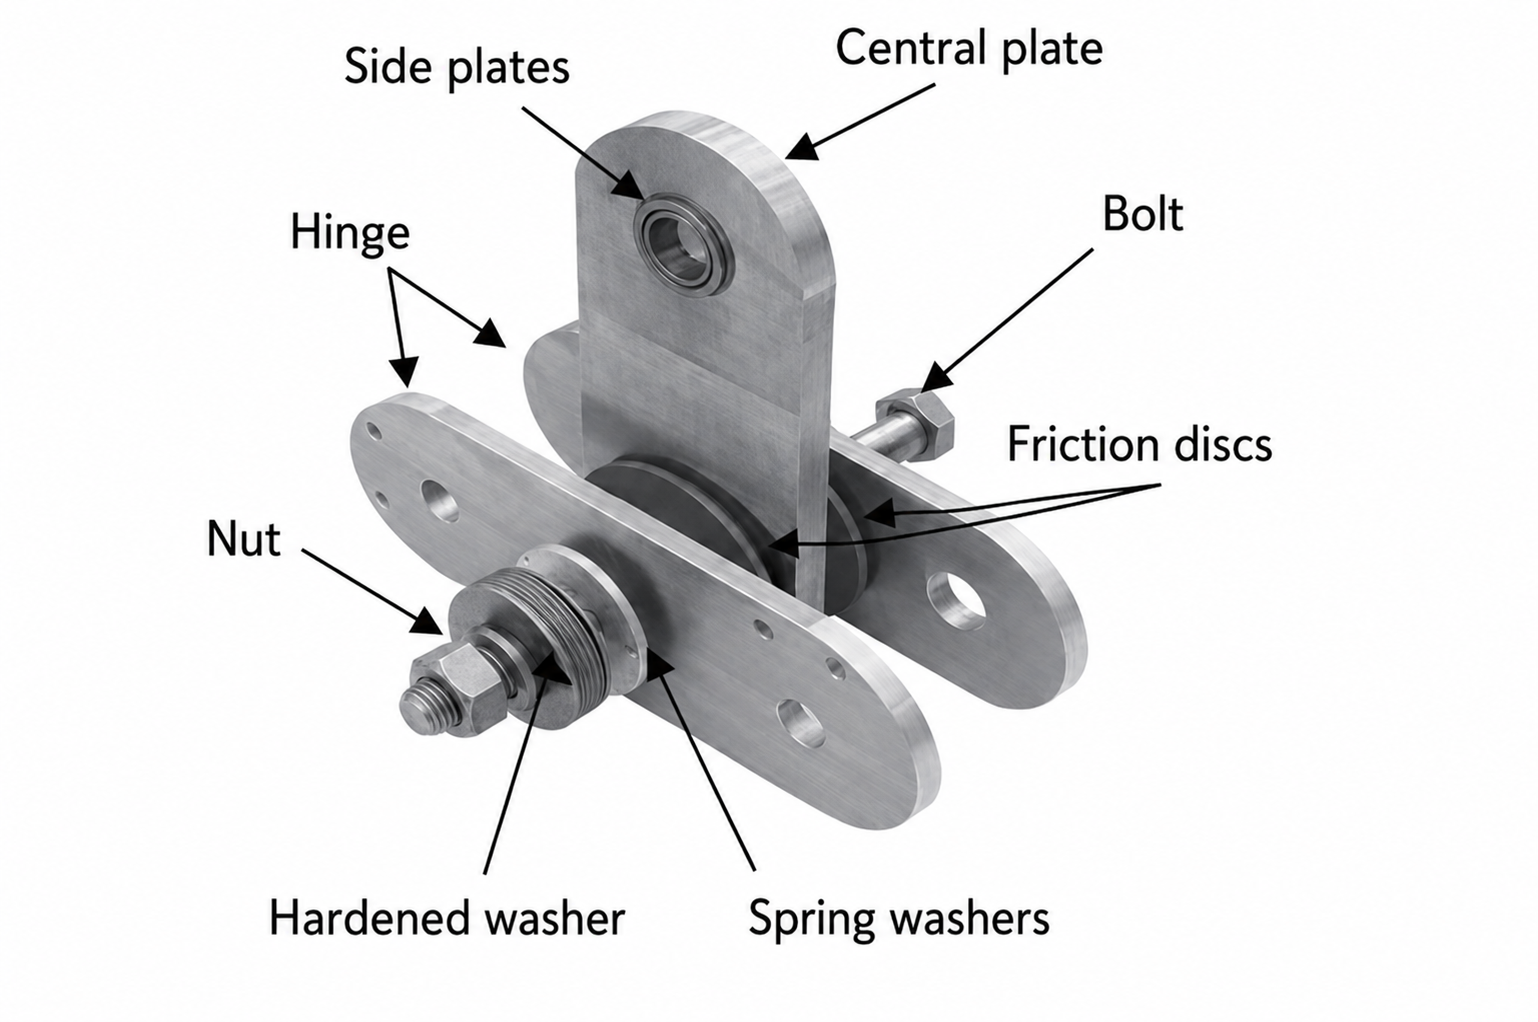
\includegraphics[width=\textwidth]{rfd_componentes.png}
        \caption{Componentes del AFR: placa central, placas laterales,
                 discos de fricción, perno pretensado y arandelas.}
        \label{fig:rfd_componentes}
    \end{subfigure}
    \hfill
    \begin{subfigure}[b]{0.48\textwidth}
        \centering
        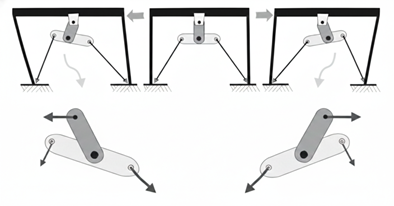
\includegraphics[width=\textwidth]{rfd_mecanismo.png}
        \caption{Mecanismo de actuación: el desplazamiento lateral del
                 marco induce la rotación en el dispositivo, disipando
                 energía por fricción.}
        \label{fig:rfd_mecanismo}
    \end{subfigure}
    \caption{Amortiguador de Fricción Rotacional (AFR). Izquierda: configuración
             física del dispositivo \citep{Mualla2002}. Derecha: secuencia de
             activación bajo excitación sísmica lateral.}
    \label{fig:rfd}
\end{figure}

En una instalación típica, la placa central del AFR se conecta al punto medio de
la viga a través de una conexión articulada, mientras que las placas laterales se
vinculan a un sistema de arriostramiento en V invertida. Cuando el marco
experimenta desplazamiento lateral debido a la excitación sísmica, el movimiento
relativo entre pisos induce la rotación en el dispositivo, como ilustra la
Figura~\ref{fig:rfd_mecanismo}. Esta rotación produce el deslizamiento entre las
placas de acero y los discos de fricción, generando un momento resistente que se
opone al movimiento. De este modo, parte de la energía que de otra forma se
disiparía mediante daño en los miembros principales del marco se transfiere al
dispositivo friccional \citep{kim_use_2011}.

La capacidad friccional del AFR se representa mediante el momento friccional
máximo $\Mf$, que depende de la fuerza normal aplicada, el coeficiente de
fricción y la geometría del dispositivo. La fuerza lateral equivalente
transferida al marco es:
\begin{equation}
    F_{\mathrm{afr}} = \frac{\Mf}{\ha},
    \label{eq:Fafr}
\end{equation}
donde $\ha$ es el brazo de palanca asociado a la geometría del sistema de
arriostramiento. Experimentalmente, \citet{Mualla2002} observaron que el
comportamiento momento--rotación del dispositivo es prácticamente independiente
de la frecuencia en el rango 2--7\,Hz, lo que apoya el uso de una ley de
fricción tipo Coulomb.

\subsection{Análisis Dinámico No Lineal mediante Dinámica No Suave}
\label{sec:theory:dns}

La fricción de Coulomb presenta una particularidad que complica su integración
numérica: el comportamiento del dispositivo cambia abruptamente entre dos
estados, deslizamiento ($|\dot{\varphi}|>0$) y adherencia ($\dot{\varphi}=0$),
sin transición continua entre ellos. Los integradores paso a paso convencionales
asumen que las fuerzas varían de manera suave entre instantes, supuesto que no
se cumple para la fricción seca \citep{chopra_dynamics_2015}. Para manejar este comportamiento sin recurrir
a linealización equivalente, en este trabajo se adopta el método de Dinámica
No Suave (DNS) propuesto por \citet{Namorado2024}, que formula el problema en
términos de velocidades e impulsos en lugar de aceleraciones y fuerzas
instantáneas.

\subsubsection*{Ley de fricción}

Para un AFR instalado entre los pisos $i$ e $i+1$, la relación entre el momento
resistente del dispositivo y la velocidad angular relativa $\dot{\varphi}_i$
sigue la ley de Coulomb:
\begin{equation}
    M_{\mathrm{afr},i} \in -\Mf \cdot \operatorname{Sign}\!\left(\dot{\varphi}_i\right),
    \label{eq:coulomb}
\end{equation}
donde $\operatorname{Sign}(\cdot)$ es el operador signo extendido al caso de
velocidad nula:
\begin{equation}
    \operatorname{Sign}(v) =
    \begin{cases}
        \{+1\}    & \text{si } v > 0, \\
        [-1,\,+1] & \text{si } v = 0, \\
        \{-1\}    & \text{si } v < 0.
    \end{cases}
    \label{eq:sign}
\end{equation}
Cuando el dispositivo desliza ($|\dot{\varphi}_i|>0$) el momento vale exactamente
$\pm\Mf$; cuando está en reposo ($\dot{\varphi}_i=0$) el momento puede tomar
cualquier valor entre $-\Mf$ y $+\Mf$ según lo exija el equilibrio estático
en ese instante.

\subsubsection*{Ecuación de movimiento}

El sistema de $\np$ pisos con $n_a$ amortiguadores instalados se rige, en su
forma continua, por la inclusión diferencial \citep{Namorado2024}:
\begin{equation}
    \bm{M}\,\ddot{\bm{u}} + \bm{C}\,\dot{\bm{u}} + \bm{K}\,\bm{u}
    \in -\bm{M}\,\bm{r}\,\ddot{x}_g(t) + \bm{H}\,\bm{Q}_f(t),
    \label{eq:eom}
\end{equation}
donde $\bm{M}$, $\bm{C}$ y $\bm{K}$ son las matrices de masa, amortiguamiento
y rigidez; $\bm{u}$ es el vector de desplazamientos relativos al suelo;
$\bm{r}$ es el vector de influencia sísmica; $\ddot{x}_g$ es la aceleración
del terreno; y $\bm{H}$ es una matriz de localización que indica en qué pisos
está instalado cada dispositivo ($+1$ en el piso superior, $-1$ en el inferior).
El símbolo $\in$ refleja que la fuerza de fricción $\bm{Q}_f(t)$ es
\textit{multivaluada}: durante el deslizamiento toma el valor $\pm\Mf/\ha$,
pero durante la adherencia puede adoptar cualquier valor en el intervalo
$[-\Mf/\ha,\,+\Mf/\ha]$ según lo exija el equilibrio, en correspondencia con
la ley de Coulomb (ec.~\ref{eq:coulomb}).

En la implementación discreta, la fuerza multivaluada $\bm{Q}_f$ se reemplaza
por los impulsos friccionales $\bm{\lambda}_{k+1}$ calculados en cada paso
mediante la resolución de un Problema de Complementariedad Lineal
(LCP, ec.~\ref{eq:lcp}). Una vez determinado
$\bm{\lambda}_{k+1}$, el valor de la fuerza queda unívocamente fijado para ese
paso y la inclusión se convierte en una igualdad:
\begin{equation}
    \bm{M}\,\ddot{\bm{u}} + \bm{C}\,\dot{\bm{u}} + \bm{K}\,\bm{u}
    = -\bm{M}\,\bm{r}\,\ddot{x}_g(t) + \bm{H}\,\bm{\lambda}_{k+1}/\Delta t.
    \label{eq:eom_disc}
\end{equation}
La fuerza equivalente recuperada para el piso $i$ es
$f_{\mathrm{afr},i} = \lambda_i / (\ha\,\Delta t)$.

\subsubsection*{Procedimiento de integración NSD-LCP-PSOR}

Partiendo del estado conocido en el instante $k$, el algoritmo calcula el
estado en $k+1$ en tres pasos que se resumen en el
Algoritmo~\ref{alg:nsd-lcp-psor}.

\textbf{Predictor.}
Se calcula primero cuál sería la velocidad del sistema si los amortiguadores
no ejercieran ninguna fuerza en este paso. Para ello se define la matriz de
masa modificada:
\begin{equation}
    \hat{\bm{M}} = \bm{M}
                  + \theta\Delta t\,\bm{C}
                  + (\theta\Delta t)^{2}\bm{K},
    \label{eq:Mhat}
\end{equation}
que agrupa en un solo operador las inercias, el amortiguamiento y la rigidez
del sistema al nivel discreto. La velocidad sin fricción es:
\begin{equation}
    \dot{\bm{u}}^{\mathrm{libre}} = \hat{\bm{M}}^{-1}
    \!\left[
        \bm{A}\,\dot{\bm{u}}_k
        - \Delta t\,\bm{K}\bm{u}_k
        - \theta\Delta t\,\bm{M}\!\left(\ddot{x}_{g,k+1}+\ddot{x}_{g,k}\right)\bm{r}
    \right],
    \label{eq:vfree}
\end{equation}
donde $\bm{A} = \bm{M} - \theta\Delta t\,\bm{C} - (\theta\Delta t)^{2}\bm{K}$.
Este resultado equivale a una integración Newmark estándar sin considerar las
fuerzas de fricción.

\textbf{Corrector.}
En general, la velocidad libre no cumple la condición de Coulomb: hay
amortiguadores que aparecen con velocidad relativa no nula cuando deberían
estar en reposo. El corrector determina los impulsos friccionales
$\bm{\lambda}_{k+1}$ necesarios para satisfacer simultáneamente la dinámica
del sistema y los límites de la ley de Coulomb. Para ello se calcula la
velocidad relativa libre en cada amortiguador,
$q_r = \dot{u}^{\mathrm{libre}}_{f_r} - \dot{u}^{\mathrm{libre}}_{f_r-1}$,
y se construye la matriz de acoplamiento entre dispositivos:
\begin{equation}
    W_{rs} = \left[\bm{H}^{\top}\hat{\bm{M}}^{-1}\bm{H}\right]_{rs}\Delta t,
    \label{eq:W}
\end{equation}
cuyos coeficientes reflejan cómo el impulso de un amortiguador afecta la
velocidad relativa de los demás a través de la estructura. Los impulsos se
obtienen resolviendo el sistema:
\begin{equation}
    \bm{W}\bm{\lambda} + \bm{q} = \bm{0},
    \quad |\lambda_r| \leq \frac{\Mf\,\Delta t}{\ha},
    \quad r = 1,\ldots,n_a,
    \label{eq:lcp}
\end{equation}
que es un Problema de Complementariedad Lineal (LCP) con restricciones de caja.
Cuando el impulso de un amortiguador alcanza el límite $\Mf\Delta t/\ha$, el
dispositivo está deslizando; cuando queda por debajo, está en reposo. El sistema
se resuelve iterativamente mediante PSOR (\textit{Projected Successive Over-Relaxation}), actualizando cada impulso en secuencia
y proyectándolo sobre el intervalo admisible hasta convergencia.

\textbf{Actualización de estado.}
Con los impulsos calculados, se corrige la velocidad y se avanza el
desplazamiento:
\begin{align}
    \dot{\bm{u}}_{k+1} &= \dot{\bm{u}}^{\mathrm{libre}}
        + \Delta t\,\hat{\bm{M}}^{-1}\bm{H}\bm{\lambda}_{k+1}, \label{eq:vupdate}\\
    \bm{u}_{k+1} &= \bm{u}_k
        + \Delta t\!\left[(1-\theta)\,\dot{\bm{u}}_k
                         + \theta\,\dot{\bm{u}}_{k+1}\right]. \label{eq:uupdate}
\end{align}
El impulso $\bm{\lambda}_{k+1}$ se reutiliza como punto de partida del PSOR
en el paso siguiente, aprovechando que la respuesta friccional cambia poco
entre instantes consecutivos.

\begin{algorithm}[t]
\caption{NSD-LCP-PSOR aplicado a marcos MDOF con AFR}
\label{alg:nsd-lcp-psor}
\begin{algorithmic}[1]
\Require $\bm{M},\bm{C},\bm{K}$; $\bm{H}$, $\bm{F}^{\lim}$;
         $\{\ddot{x}_{g,k}\}_{k=0}^{n}$; $\Delta t$, $\theta$
\Ensure  $\{\bm{u}_k,\dot{\bm{u}}_k\}_{k=0}^{n}$

\vspace{2pt}
\State \textit{// Pre-cómputo (una sola vez)}
\State $\hat{\bm{M}} \leftarrow \bm{M} + \theta\Delta t\,\bm{C} + (\theta\Delta t)^{2}\bm{K}$
\State $\bm{A} \leftarrow \bm{M} - \theta\Delta t\,\bm{C} - (\theta\Delta t)^{2}\bm{K}$
\State $\bm{W} \leftarrow \left(\bm{H}^{\top}\hat{\bm{M}}^{-1}\bm{H}\right)\Delta t$
\State $\bm{u}_0 \leftarrow \bm{0}$;\quad $\dot{\bm{u}}_0 \leftarrow \bm{0}$;\quad
       $\bm{\lambda}_0 \leftarrow \bm{0}$

\vspace{2pt}
\For{$k = 0, 1, \ldots, n-1$}
    \vspace{2pt}
    \State \textit{// Paso 1 — velocidad libre (predictor sin fricción)}
    \State $\bm{b}_k \leftarrow \bm{A}\,\dot{\bm{u}}_k
            - \Delta t\,\bm{K}\bm{u}_k
            - \theta\Delta t\,\bm{M}
              \!\left(\ddot{x}_{g,k+1}+\ddot{x}_{g,k}\right)\bm{r}$
    \State $\dot{\bm{u}}^{\mathrm{lib}} \leftarrow \hat{\bm{M}}^{-1}\bm{b}_k$

    \vspace{2pt}
    \State \textit{// Paso 2 — velocidades relativas libres en cada amortiguador}
    \State $q_r \leftarrow \dot{u}^{\mathrm{lib}}_{f_r} - \dot{u}^{\mathrm{lib}}_{f_r-1}$
           \quad para $r = 1,\ldots,n_a$

    \vspace{2pt}
    \State \textit{// Paso 3 — resolución del LCP por PSOR (corrector)}
    \State $\bm{\lambda}^{(0)} \leftarrow \bm{\lambda}_k$
           \quad\textit{(punto de partida desde el paso anterior)}
    \While{$\|\bm{\lambda}^{(i+1)} - \bm{\lambda}^{(i)}\|_\infty > \varepsilon$}
        \For{$r = 1,\ldots,n_a$}
            \State $\tilde{\lambda}_r \leftarrow
                   -\!\left(q_r + \sum_{s \neq r} W_{rs}\lambda_s^{(i)}\right)\!\big/W_{rr}$
            \State $\lambda_r^{(i+1)} \leftarrow
                   \max\!\left(-F^{\lim}_r,\;\min\!\left(F^{\lim}_r,\;\tilde{\lambda}_r\right)\right)$
        \EndFor
    \EndWhile
    \State $\bm{\lambda}_{k+1} \leftarrow \bm{\lambda}^{(*)}$
           \quad\textit{($F^{\lim}_r = \Mf\Delta t/\ha$)}

    \vspace{2pt}
    \State \textit{// Paso 4 — actualización de estado}
    \State $\dot{\bm{u}}_{k+1} \leftarrow
           \dot{\bm{u}}^{\mathrm{lib}} +
           \Delta t\,\hat{\bm{M}}^{-1}\bm{H}\bm{\lambda}_{k+1}$
    \State $\bm{u}_{k+1} \leftarrow \bm{u}_k +
           \Delta t\!\left[(1-\theta)\,\dot{\bm{u}}_k +
                           \theta\,\dot{\bm{u}}_{k+1}\right]$
\EndFor
\end{algorithmic}
\end{algorithm}

El paso de tiempo utilizado, $\Delta t = 0{,}01$\,s, corresponde al intervalo
de muestreo nativo de los registros sísmicos, lo que evita interpolación de
la señal de entrada. Para las estructuras más rígidas del experimento
($T_1 = 0{,}3$\,s) esto representa aproximadamente 30 puntos de integración
por período, satisfaciendo el criterio estándar $\Delta t / T_1 \leq 0{,}10$
recomendado para métodos de Newmark \citep{chopra_dynamics_2015}.
La fuerza friccional equivalente en el piso $i$ se recupera como:
\begin{equation}
    f_{\mathrm{afr},i} = \frac{\lambda_i}{\ha\,\Delta t},
    \label{eq:ffrict}
\end{equation}
de modo que el estado de deslizamiento o adherencia de cada dispositivo queda
determinado automáticamente por la solución del LCP, sin necesidad de
detectarlo de forma explícita.

\subsubsection*{Adaptación del método DNS para simulación masiva MDOF}
\label{sec:theory:nsd:adaptacion}

El método DNS de \citet{Namorado2024} fue desarrollado y validado para marcos
de uno a cinco pisos con un amortiguador por piso. En este trabajo se aplica
a marcos de hasta veinte pisos con configuraciones variables de amortiguadores,
lo que requirió tres ajustes al algoritmo original.

\textbf{Formulación LCP del corrector.}
En lugar de actualizar los impulsos de cada amortiguador por separado en
secuencia, se resuelven todos de forma conjunta mediante la matriz $\bm{W}$
(ec.~\ref{eq:W}), que recoge cómo interactúan los distintos dispositivos a
través de la estructura. Esto resulta más directo cuando hay varios
amortiguadores activos simultáneamente en pisos distintos, aunque requiere
calcular $\hat{\bm{M}}^{-1}$ una vez antes de iniciar la integración.

\textbf{Sin parámetro de ajuste.}
El algoritmo original incluye un parámetro $\alpha$ que controla la velocidad
de convergencia del corrector y que debe elegirse para cada caso. Al formular
el problema como LCP, ese parámetro desaparece: el procedimiento iterativo
converge sin ajuste manual, lo que facilita su aplicación a las miles de
configuraciones distintas del experimento.

\textbf{Reutilización del impulso entre pasos.}
El impulso calculado en el paso $k$ se usa como punto de partida en el paso
$k+1$. Dado que la respuesta del sistema cambia gradualmente, este valor
inicial suele estar cerca de la solución, por lo que se necesitan menos
iteraciones para converger.

En términos físicos, las dos formulaciones son equivalentes: ambas resuelven
la misma ley de fricción de Coulomb discreta. La diferencia está en cómo se
organiza el cálculo para manejar de forma eficiente el mayor número de pisos
y amortiguadores de este estudio.

\subsection{Métrica de Desempeño Sísmico}
\label{sec:theory:metrica}

El desempeño sísmico de cada configuración de AFR se cuantifica mediante
razones de respuesta normalizadas respecto a la estructura de referencia sin
amortiguadores, enfoque consistente con trabajos previos sobre AFR
\citep{Namorado2024, Jarrahi2020jbe, Mualla2002}. Para cada par configuración--registro
se calculan tres razones:
\begin{equation}
    R_1 = \frac{u_{\max}^{(\mathrm{c})}}{u_{\max}^{(0)}}, \quad
    R_2 = \frac{\ddot{u}_{\max}^{(\mathrm{c})}}{\ddot{u}_{\max}^{(0)}}, \quad
    R_3 = \frac{V_{\max}^{(\mathrm{c})}}{V_{\max}^{(0)}},
    \label{eq:R_individual}
\end{equation}
donde los superíndices (c) y (0) denotan la estructura controlada y la no
controlada, respectivamente; $u_{\max}$ es el desplazamiento máximo de cubierta,
$\ddot{u}_{\max}$ es la aceleración absoluta máxima y $V_{\max}$ es el cortante
basal máximo. A partir de $R_1$, $R_2$ y $R_3$ se construyen dos índices compuestos
mediante la norma euclídea. El primero combina desplazamiento y aceleración:
\begin{equation}
    CR_1 = \sqrt{R_1^2 + R_2^2},
    \label{eq:CR1}
\end{equation}
y el segundo agrega el cortante basal, integrando los tres aspectos de la
respuesta simultáneamente:
\begin{equation}
    CR_2 = \sqrt{R_1^2 + R_2^2 + R_3^2}.
    \label{eq:CR2}
\end{equation}
Cuando los amortiguadores no tienen efecto, $R_1 = R_2 = R_3 = 1$ y por tanto
$CR_2 = \sqrt{3}$; valores menores indican que la configuración reduce la
respuesta sísmica en alguna combinación de las tres medidas.

Dado que la respuesta sísmica depende del registro considerado, $CR_2$ se calcula
para cada par configuración--registro. Siguiendo la práctica estándar de la
evaluación sísmica basada en desempeño \citep{Kazemi2022}, el valor de $CR_2$ se
resume sobre los $N_r = 8$ registros mediante tres estadísticos percentilares:
\begin{align}
    \CR{P10} &= Q_{0{,}10}\!\left(\{CR_2^{(k)}\}_{k=1}^{N_r}\right), \quad
    \CR{med}  = Q_{0{,}50}\!\left(\{CR_2^{(k)}\}_{k=1}^{N_r}\right), \notag\\
    \CR{P90} &= Q_{0{,}90}\!\left(\{CR_2^{(k)}\}_{k=1}^{N_r}\right),
    \label{eq:CR2stats}
\end{align}
donde $Q_p$ denota el cuantil de orden $p$. Estos tres estadísticos sirven como
variables objetivo de los modelos ML. La interpretación es: $\CR{P10}$
representa una condición favorable de la respuesta, $\CR{med}$ describe el
comportamiento típico y $\CR{P90}$ aproxima una condición severa dentro del
conjunto de registros, permitiendo distinguir configuraciones que solo funcionan
adecuadamente ante un registro particular de aquellas con desempeño estable
frente a la variabilidad sísmica.

\subsection{Aprendizaje Automático para Optimización Estructural}
\label{sec:theory:ml}

La optimización de sistemas de disipación pasiva implica la búsqueda de la
combinación óptima de ubicación, número y capacidad de los dispositivos para
minimizar algún indicador de respuesta sísmica. Enfoques previos han abordado
este problema mediante métodos energéticos y algoritmos metaheurísticos aplicados
a amortiguadores de fricción convencionales y rotacionales
\citep{moreschi_design_2003, moghaddam_optimal_2022, ontiveros-perez_reliability-based_2019}.
El aprendizaje automático permite construir modelos sustituto que aproximan la
relación entrada--salida del análisis no lineal con un costo computacional
significativamente menor, lo que habilita la exploración eficiente de espacios
de diseño de alta dimensión.

En el paradigma del modelo sustituto, se entrena una función de regresión
$\hat{y} = f(\bm{x};\,\bm{\theta})$ sobre datos $\{(\bm{x}_i,\,y_i)\}_{i=1}^{N}$
para aproximar el mapeo entre las variables de diseño $\bm{x}$ (parámetros
estructurales y de AFR) y la variable objetivo $y$ (uno de los tres estadísticos
de $CR_2$). El entrenamiento minimiza el error cuadrático medio:
\begin{equation}
    \mathcal{L}(\bm{\theta}) = \frac{1}{N}\sum_{i=1}^{N}
    \bigl(y_i - f(\bm{x}_i;\,\bm{\theta})\bigr)^2.
    \label{eq:mse}
\end{equation}

Se comparan cuatro algoritmos: (i)~Regresión Lineal y (ii)~Regresión Ridge
(penalización $\ell_2$) como referencias lineales; (iii)~Random Forest
\citep{Breiman2001}, que promedia predicciones de múltiples árboles entrenados
de forma independiente; y (iv)~XGBoost \citep{Chen2016}, un algoritmo de
\textit{gradient boosting} que corrige secuencialmente los residuales de un
ensemble creciente. La generalización se estima mediante validación cruzada
GroupKFold de cinco particiones \citep{Kazemi2022}, donde los grupos corresponden
a identificadores de estructura únicos. Esta estrategia previene que distintas
configuraciones del mismo edificio ---que comparten propiedades dinámicas y por
tanto respuestas correlacionadas--- aparezcan simultáneamente en entrenamiento
y validación, evitando la sobreestimación del desempeño predictivo por fuga
de información entre particiones. Las métricas de evaluación son:
\begin{equation}
    \RMSE = \sqrt{\frac{1}{|V|}\sum_{i \in V}\bigl(y_i - \hat{y}_i\bigr)^2},
    \qquad
    \Rsq  = 1 - \frac{\sum_{i \in V}(y_i - \hat{y}_i)^2}
                      {\sum_{i \in V}(y_i - \bar{y})^2},
    \label{eq:metrics}
\end{equation}
donde $V$ es el conjunto de validación, $\hat{y}_i$ son predicciones fuera de la
muestra de entrenamiento (\textit{out-of-fold}) y $\bar{y}$ es la media de los
valores observados.

%%═══════════════════════════════════════════════════════════════════════════
\section{Metodología}
\label{sec:method}
%%═══════════════════════════════════════════════════════════════════════════

\subsection{Diseño de Experimentos}
\label{sec:method:doe}

Se utilizó un Muestreo por Hipercubo Latino (MHL) \citep{McKay1979} para generar
1\,000 marcos tipo cortante estructuralmente diversos. Cada configuración queda
definida por cinco variables estructurales: número de pisos $\np \in \{3, 5, 7,
10, 12, 15, 18, 20\}$; período fundamental objetivo $T_1 \in [0{,}3,\,3{,}0]$\,s;
masa promedio por nivel $\bar{m} \in [150,\,350]$\,t/piso; perfil de distribución
de masa (uniforme, ascendente lineal, descendente lineal o concentrada en parte
alta); y perfil de rigidez lateral (uniforme, ascendente lineal, descendente
lineal o piso suave en la base). La rigidez lateral se calibró analíticamente
para satisfacer el $T_1$ objetivo mediante el problema de valores propios
generalizado $(\bm{K} - \omega_1^2\,\bm{M})\,\bm{\phi}_1 = \bm{0}$, con
$\omega_1 = 2\pi/T_1$.

Para cada estructura se generaron $\approx 50$ configuraciones de AFR: 40
mediante MHL sobre el espacio binario de ubicación y el rango de momento
friccional $\Mf \in [25,\,500]$\KM, y 10 configuraciones estructuradas
orientadas a fracciones de cobertura específicas. La configuración se codifica
mediante un vector binario $\bm{b} \in \{0,1\}^{\np}$, donde $b_i = 1$ indica
la presencia de un AFR en el piso $i$, obteniéndose el número de amortiguadores
$\nd = \|\bm{b}\|_0$ y la densidad de cobertura $\etad = \nd/\np \in (0,\,1]$.
El plan experimental total comprende 433\,984 simulaciones
($\approx 1\,000 \times 54 \times 8$).

\subsection{Modelos Estructurales y Análisis Dinámico}
\label{sec:method:modelo}

Cada estructura se modela como un marco cortante lineal con masas concentradas
por nivel y rigidez lateral entre pisos. La matriz de masa diagonal es
$\bm{M} = \mathrm{diag}(m_1,\ldots,m_{\np})$ y la matriz de rigidez tridiagonal
$\bm{K}$ se ensambla a partir del vector de rigidez entre pisos $k_i$.
Se adopta amortiguamiento de Rayleigh con razón $\zeta = 3\,\text{\%}$, calibrado a
los modos 1 y 3 \citep{chopra_dynamics_2015}. Los ocho acelerogramas reales que constituyen la demanda sísmica
son: El~Centro~1940, Jamiltepec~2018, Kobe~1995, Loma Prieta~1989, Niltepec~2017,
Northridge~1994, Trinidad~1983 y Zacatula~1997. La integración tiempo-historia sigue el esquema de punto medio DNS
\citep{Namorado2024} con paso de tiempo $\Delta t = 0{,}01$\,s, igual al
intervalo de muestreo nativo de los registros. El brazo de palanca se fija en
$\ha = 0{,}40$\,m, valor dentro del rango reportado en la literatura para
marcos de acero con AFR \citep{Mualla2002, Jarrahi2020jbe}.

\subsection{Ingeniería de Características}
\label{sec:method:features}

Las cuatro variables de diseño primarias no capturan la información espacial
de la configuración de AFR ni las relaciones de escala entre parámetros; un
modelo de árboles entrenado únicamente sobre ellas tendría que inferir cocientes
y posiciones a partir de sus componentes, lo que incrementa la profundidad
requerida y puede degradar la generalización. Se calculan, por tanto, cinco
características derivadas que compactan esta información de forma explícita.

El vector de características completo contiene 29 predictores distribuidos en
tres grupos:

\begin{enumerate}[label=\textit{\roman*})]
    \item \textbf{Variables de diseño primarias} (4):
          número de pisos $\np$, período fundamental objetivo $T_1$,
          momento de fricción $\Mf$ y número de amortiguadores $\nd$.

    \item \textbf{Características derivadas} (5):
    \begin{itemize}
        \item $\etad = \nd/\np$: densidad de amortiguadores, variable de
              diseño dominante según el análisis de importancia
              (Sección~\ref{sec:results:importancia});
        \item $\bar{p} = \tfrac{1}{\nd}\sum_{i:\,b_i=1} i$: posición
              promedio de los dispositivos en número de piso;
        \item $\tilde{p} = \bar{p}/\np \in (0,\,1]$: posición promedio
              normalizada, indicadora de si los AFR se concentran en pisos
              bajos o altos;
        \item $\sigma_p = \mathrm{std}\!\left(\{i:b_i=1\}\right)/\np$:
              dispersión vertical normalizada, que distingue configuraciones
              uniformes de agrupadas;
        \item $\tilde{E} = E_{\mathrm{total}}/(\np\times10^6)$: energía
              disipada total normalizada por piso, proxy de la demanda
              dinámica integrada.
    \end{itemize}

    \item \textbf{Indicadores binarios de ubicación} (20):
          $b_1,\ldots,b_{20}$, donde $b_i=1$ si el piso $i$ cuenta con
          un AFR y $b_i=0$ en caso contrario; marcos con menos de 20 pisos
          se rellenan con ceros.
\end{enumerate}

\subsection{Entrenamiento y Validación}
\label{sec:method:entrenamiento}

Los objetivos $\CR{med}$, $\CR{P10}$ y $\CR{P90}$ se predicen de forma
independiente. Para cada objetivo, los cuatro algoritmos se entrenan y evalúan
mediante validación cruzada GroupKFold de cinco particiones. Los
hiperparámetros se fijan en valores estándar: Random Forest usa $n=100$ árboles
y profundidad máxima 15; XGBoost usa $n=100$ estimadores, profundidad máxima 6
y tasa de aprendizaje $\eta=0{,}1$. La importancia de características se deriva
del decremento medio de impureza en todos los árboles del modelo XGBoost
entrenado. Las predicciones fuera de muestra (\textit{out-of-fold}, OOF) se
ensamblan entre particiones para calcular los valores reportados de $\RMSE$ y
$\Rsq$.

%%═══════════════════════════════════════════════════════════════════════════
\section{Resultados}
\label{sec:results}
%%═══════════════════════════════════════════════════════════════════════════

\subsection{Desempeño Predictivo de los Modelos ML}
\label{sec:results:desempenio}

La \cref{tab:desempenio} presenta el RMSE y $R^2$ con validación cruzada para
todos los modelos y objetivos. Los modelos de ensemble logran una reducción del
49\,\% en $\RMSE$ respecto a los baselines lineales para $\CR{med}$, y del
40\,\% para $\CR{P10}$. XGBoost obtiene el menor error en $\CR{med}$ y $\CR{P10}$, mientras que
Random Forest presenta una pequeña ventaja en $\CR{P90}$
(\cref{fig:comparacion_modelos}).

\begin{table}[h!]
\centering
\caption{RMSE y $R^2$ con validación cruzada por modelo y variable objetivo.
         GroupKFold de cinco particiones, agrupadas por identificador de
         estructura.}
\label{tab:desempenio}
\small
\setlength{\tabcolsep}{4pt}
\begin{tabular}{lcccccc}
\toprule
& \multicolumn{2}{c}{$\CR{med}$}
& \multicolumn{2}{c}{$\CR{P10}$}
& \multicolumn{2}{c}{$\CR{P90}$} \\
\cmidrule(lr){2-3}\cmidrule(lr){4-5}\cmidrule(lr){6-7}
Modelo & $\RMSE$ & $\Rsq$ & $\RMSE$ & $\Rsq$ & $\RMSE$ & $\Rsq$ \\
\midrule
Regresión Lineal & 0{,}1274 & 0{,}695 & 0{,}1267 & 0{,}812 & 0{,}1838 & 0{,}435 \\
Ridge            & 0{,}1274 & 0{,}695 & 0{,}1268 & 0{,}812 & 0{,}1838 & 0{,}435 \\
Random Forest    & 0{,}0681 & 0{,}913 & 0{,}0785 & 0{,}928 & 0{,}0981 & \textbf{0{,}839} \\
XGBoost          & \textbf{0{,}0652} & \textbf{0{,}920} & \textbf{0{,}0755} & \textbf{0{,}933} & 0{,}0984 & 0{,}838 \\
\bottomrule
\end{tabular}
\end{table}

\begin{figure}[htbp]
\centering
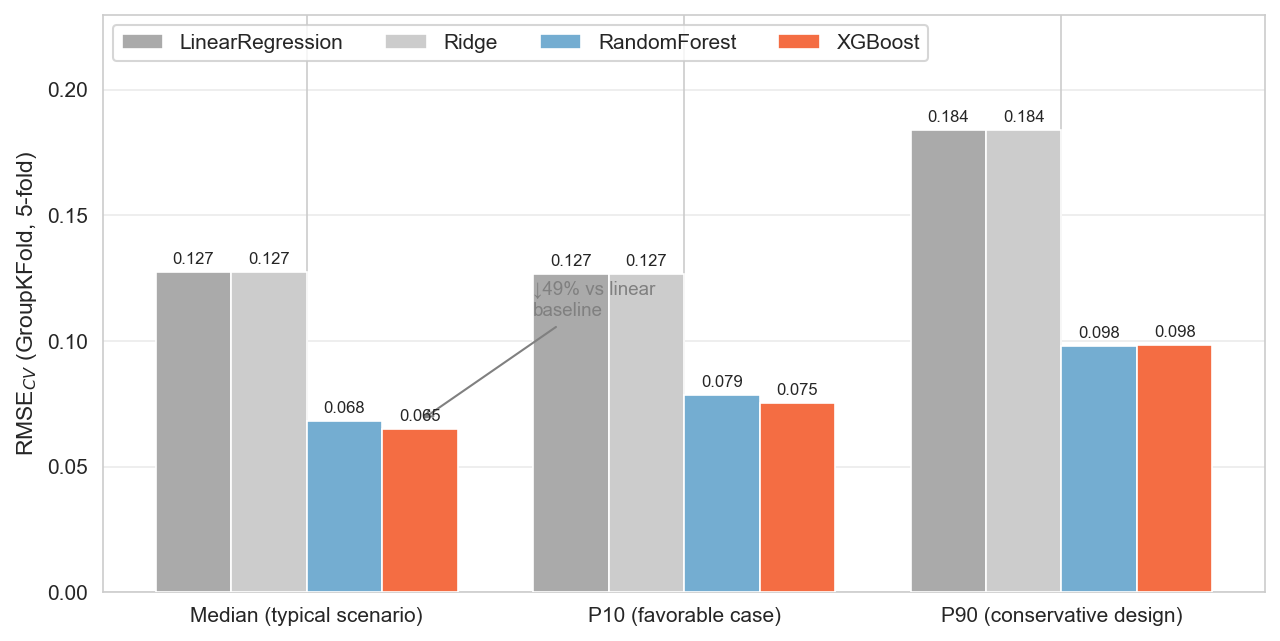
\includegraphics[width=0.85\linewidth]{figs/F1_model_comparison_rmse.png}
\caption{Comparación del $\RMSE$ con validación cruzada entre modelos y variables
objetivo. Los modelos de ensemble alcanzan aproximadamente la mitad del error de
los baselines lineales.}
\label{fig:comparacion_modelos}
\end{figure}

Para $\CR{P10}$ los modelos lineales alcanzan $\Rsq = 0{,}81$, lo que indica
que en los escenario favorables, la relación entre predictores y respuesta es
predominantemente lineal. El $\Rsq = 0{,}44$ sustancialmente menor
para $\CR{P90}$ bajo modelos lineales confirma que el escenario conservador está
gobernado por interacciones no lineales que solo los modelos de ensemble pueden
capturar.

La \cref{fig:pred_vs_actual} muestra la dispersión OOF de XGBoost sobre
$\CR{med}$, junto con el análisis de residuales. Las predicciones se distribuyen
estrechamente alrededor de la línea de identidad sin sesgo sistemático. Se
observa un ligero incremento en la magnitud de los residuales para
$CR_2 > 1{,}8$, zona dominada por marcos bajos ($\np \leq 5$); en estos casos
la respuesta estructural es más sensible a variaciones pequeñas en los
parámetros de diseño, lo que incrementa la variabilidad intrínseca del target
y dificulta la predicción.

\begin{figure}[htbp]
\centering
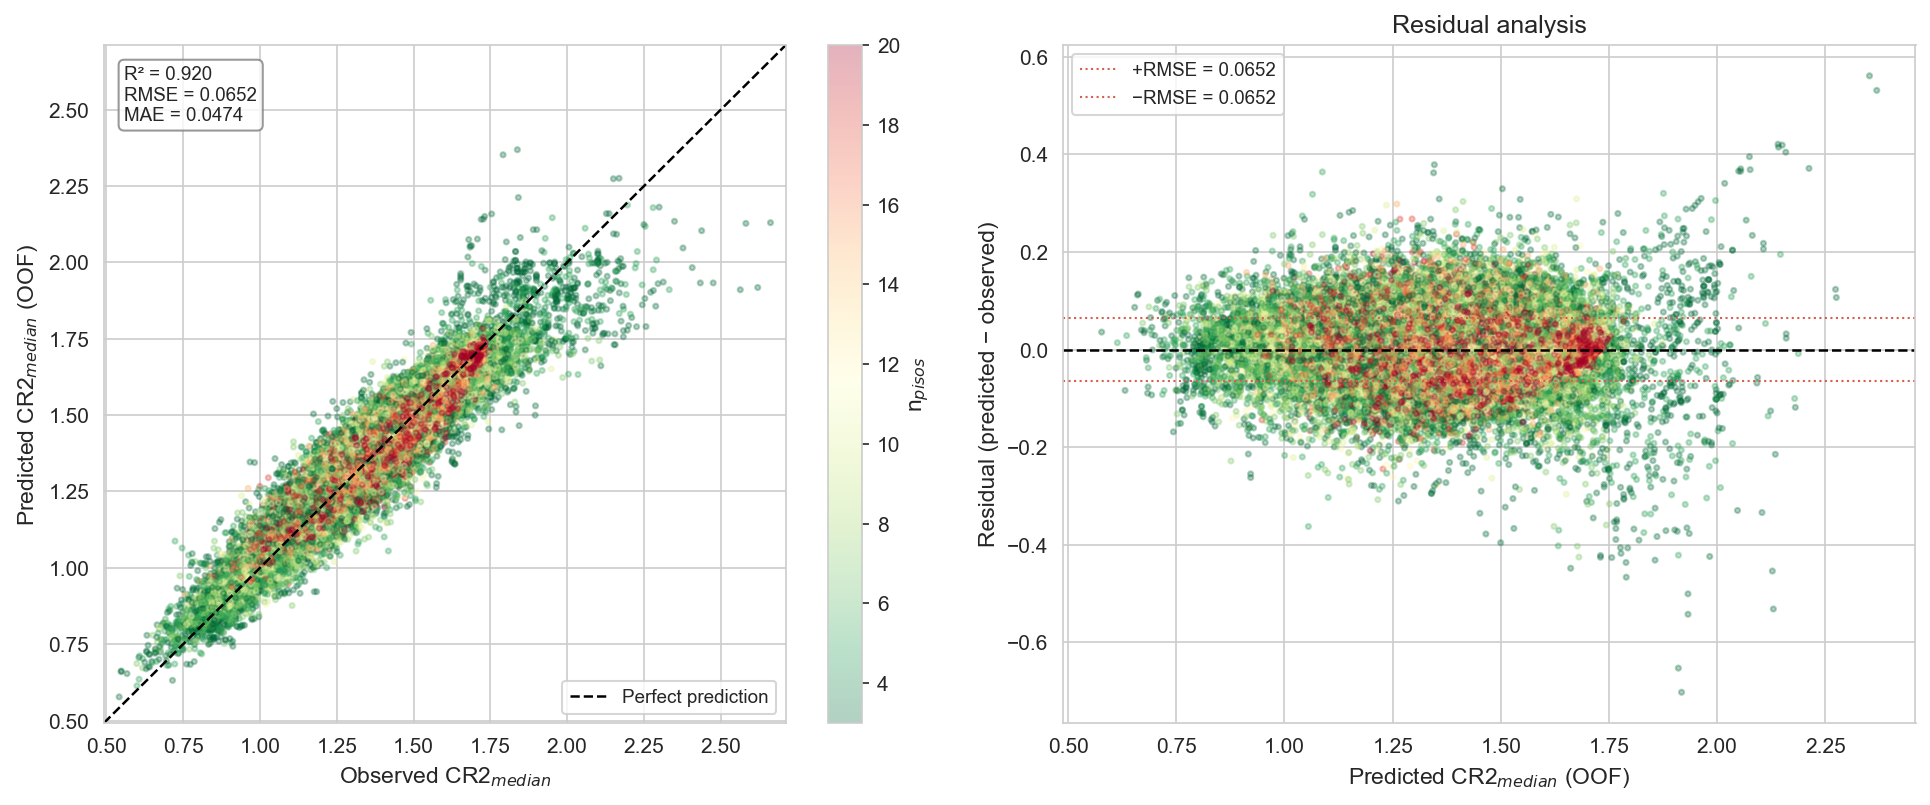
\includegraphics[width=\linewidth]{figs/F2_predicted_vs_actual_oof.png}
\caption{XGBoost OOF para $\CR{med}$. \textit{Izquierda}: predicción vs.\
valor observado; línea punteada: predicción perfecta; color: $\np$.
\textit{Derecha}: residuales (predicho $-$ observado) vs.\ predicho;
bandas punteadas: $\pm\RMSE$. $\Rsq = 0{,}92$, $\RMSE = 0{,}065$.}
\label{fig:pred_vs_actual}
\end{figure}

\begin{figure}[htbp]
\centering
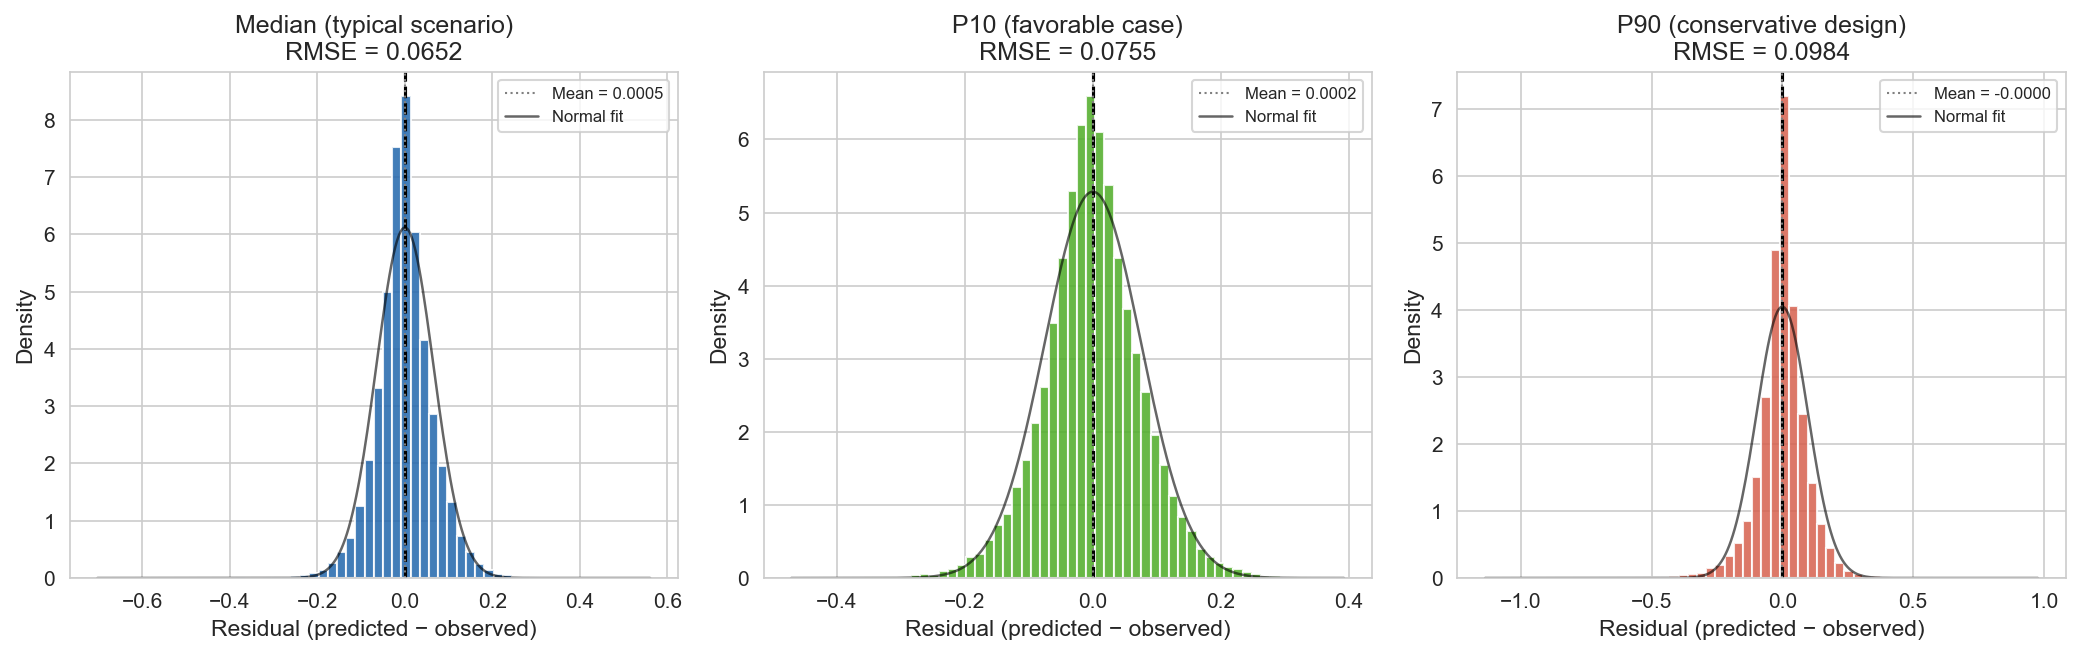
\includegraphics[width=\linewidth]{figs/F3_residual_distributions.png}
\caption{Distribuciones de residuales (OOF, XGBoost) para las tres variables
objetivo de $CR_2$. Línea punteada: referencia de media cero; curva sólida:
ajuste normal.}
\label{fig:residuales}
\end{figure}

\subsection{Jerarquía de Variables de Diseño e Importancia de Características}
\label{sec:results:importancia}

La \cref{fig:importancia} presenta las 12 características más relevantes para
cada variable objetivo, derivadas del modelo XGBoost. En los tres escenarios, la
densidad de amortiguadores $\etad$ ocupa consistentemente el primer lugar, con
una correlación de Pearson $r = -0{,}73$ con $\CR{med}$, frente a $r = -0{,}45$
del número absoluto $\nd$.

La energía disipada normalizada $\tilde{E}$ ($r = -0{,}70$) y la dispersión
vertical $\sigma_p$ ($r = -0{,}54$) ocupan el segundo y tercer lugar,
respectivamente, y están estrechamente vinculadas: una distribución homogénea
de los dispositivos a lo largo de la altura favorece una disipación de energía
más uniforme entre pisos, reduciendo la concentración de demanda en niveles
específicos. En particular, configuraciones que incluyen
los pisos inferiores ---donde la deriva entre pisos es típicamente mayor---
resultan más eficientes, resultado consistente con \citet{aydin_simple_2013}
y con los hallazgos de optimización de colocación reportados por
\citet{moghaddam_optimal_2022} y \citet{miguel_simultaneous_2016}. El momento friccional
$\Mf$ muestra una correlación marginal más débil ($r = -0{,}19$) de forma
aislada, pero interactúa fuertemente con $\etad$, como se muestra en la
\cref{sec:results:interaccion}.

Una diferencia notable entre escenarios es el comportamiento de $\CR{P90}$:
la densidad global $\etad$ pierde su posición dominante (rank~1 en mediana y
P10, rank~4 en P90) y son sustituida por la presencia específica de
amortiguadores en los pisos~1 y~2 junto con la altura del edificio $\np$,
que pasan a ocupar los tres primeros lugares. Esto indica que bajo los
registros más demandantes, la ubicación precisa en los niveles inferiores y
las características de la estructura cobran mayor relevancia que la cobertura
global.

\begin{figure}[htbp]
\centering
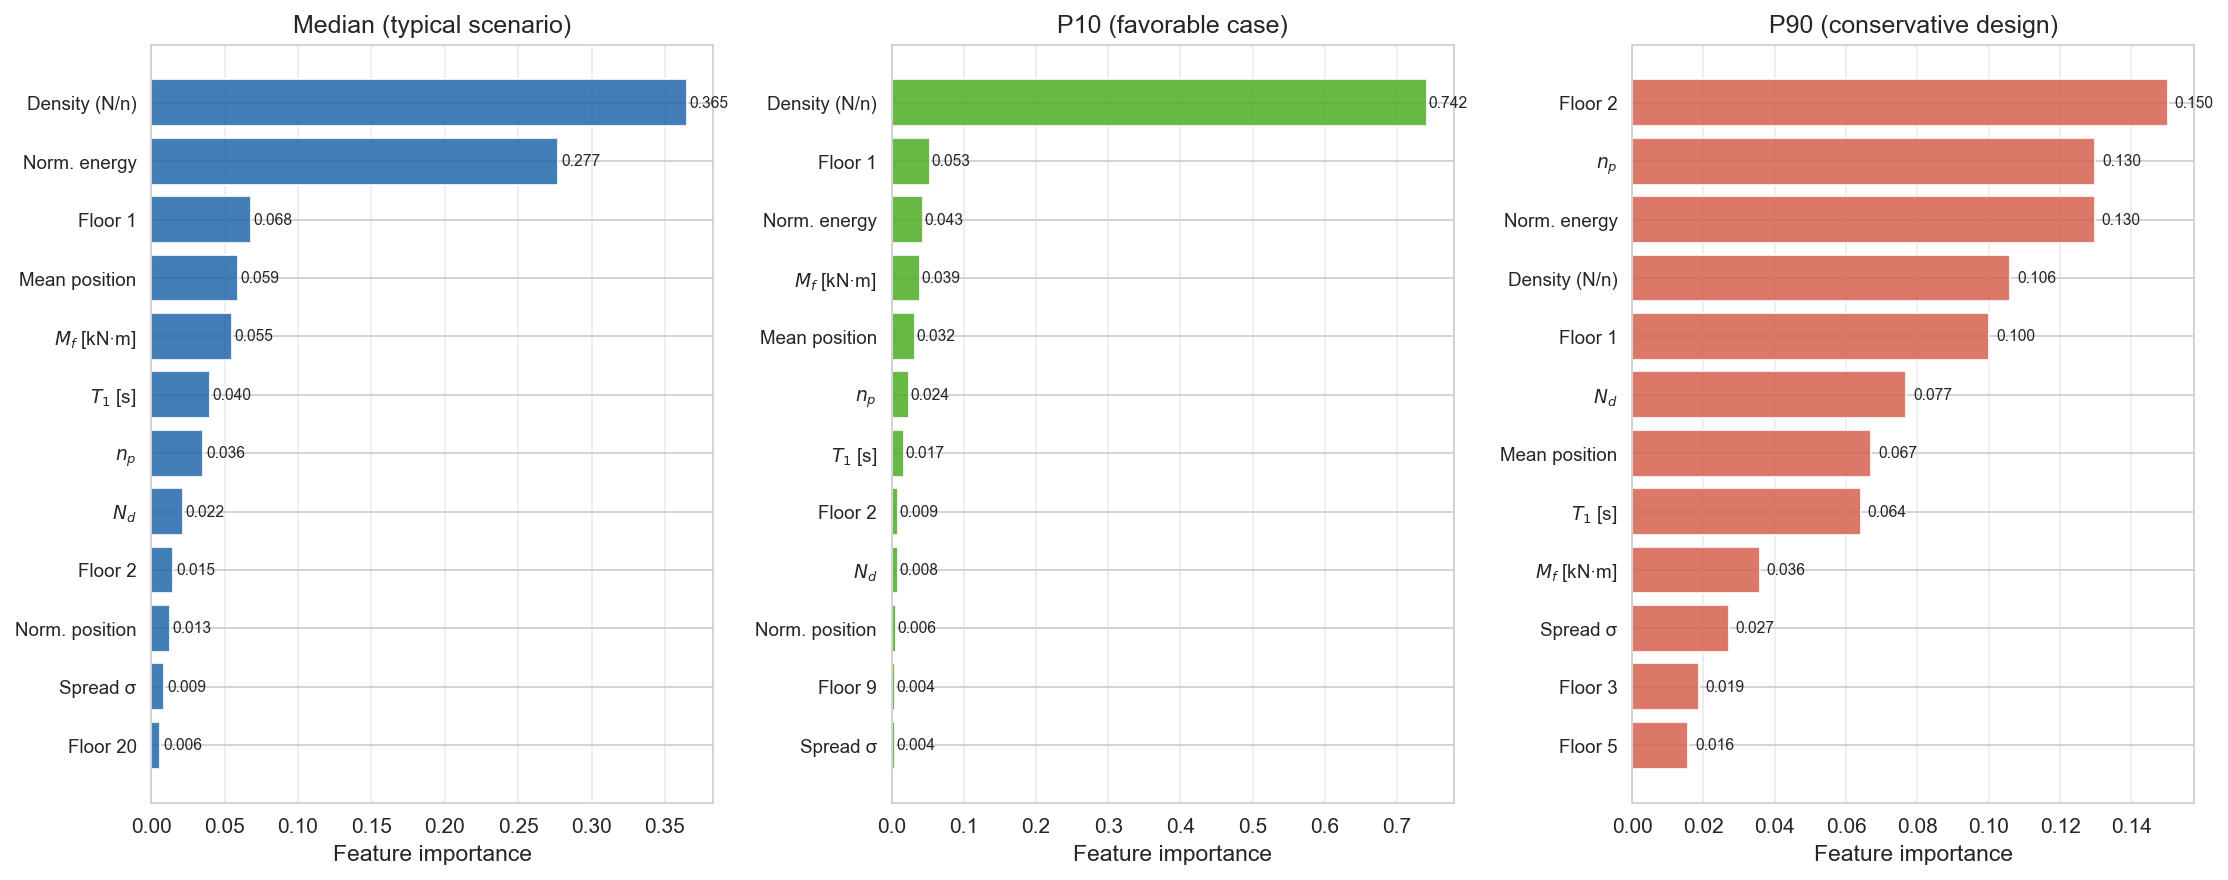
\includegraphics[width=\linewidth]{figs/F4_feature_importance_3targets.png}
\caption{Importancia de características (XGBoost) para los 12 predictores
principales en los tres escenarios de $CR_2$. Las barras horizontales indican el
decremento medio de impureza, normalizado dentro de cada modelo. Nota: los ejes
horizontales de cada panel tienen escalas independientes; la comparación entre
escenarios debe hacerse por orden de importancia relativa, no por magnitud
absoluta.}
\label{fig:importancia}
\end{figure}

\subsection{Rendimiento Decreciente: Efecto de la Densidad de Amortiguadores}
\label{sec:results:decreciente}

La \cref{fig:decreciente} investiga la relación de rendimiento decreciente entre
$\etad$ y $CR_2$. Para cada estructura se identificó el mejor $\CR{med}$
alcanzable para cada valor de $\nd$, seleccionando el mínimo $CR_2$ entre todas
las configuraciones que comparten ese conteo. Las curvas de desempeño se
estratifican por altura del edificio para eliminar el efecto de confusión de
$\np$ sobre el eje de $\nd$ absoluto.

Las curvas confirman un patrón de rendimiento decreciente consistente en todas
las categorías de altura, con la mejora más pronunciada en el rango
$\etad \in [0{,}30,\,0{,}60]$. Más allá de $\etad = 0{,}60$, la ganancia
marginal por piso adicional cubierto disminuye monotónicamente. Un análisis de
umbral basado en la ganancia normalizada intra-estructura
(\cref{fig:curvas_internas}) indica que el 80\,\% de la mejora máxima de
desempeño se alcanza con $\etad \approx 0{,}85$ para marcos de mediana altura
(6--10 pisos), alta altura (11--15 pisos) y altura considerable (16--20 pisos).
Los marcos de baja altura (3--5 pisos) requieren $\etad \approx 0{,}95$ para
alcanzar el mismo umbral del 80\,\%, lo que se atribuye al impacto
proporcionalmente mayor de cada dispositivo adicional en edificios con pocos
pisos.

Para verificar si esta dominancia de $\etad$ se mantiene con independencia de
las demás variables de diseño, se realizó un análisis de dominancia estocástica
sobre los ocho registros sísmicos por separado. En cada registro se comparó el
percentil~5 (mejor 5\,\%) de $CR_2$ en un intervalo de densidad superior contra
el percentil~95 (peor 5\,\%) del intervalo inmediatamente inferior. La
dominancia se confirma en los ocho registros: incluso una configuración
desfavorable en $\Mf$, posición o $T_1$, pero con mayor densidad de cobertura,
supera al 95\,\% de las configuraciones con densidad inferior. La correlación
de Pearson entre $\etad$ y $CR_2$ varía de $r=-0{,}74$ (El~Centro~1940) a
$r=-0{,}55$ (Kobe~1995) para la mayoría de los registros. La excepción es
Trinidad~1983 ($r=-0{,}18$), donde la correlación con la densidad se debilita
notablemente y las variables de posición y capacidad por dispositivo recuperan
relevancia, lo que sugiere que registros de baja intensidad o contenido
frecuencial atípico pueden reducir la dominancia de $\etad$.

\begin{figure}[htbp]
\centering
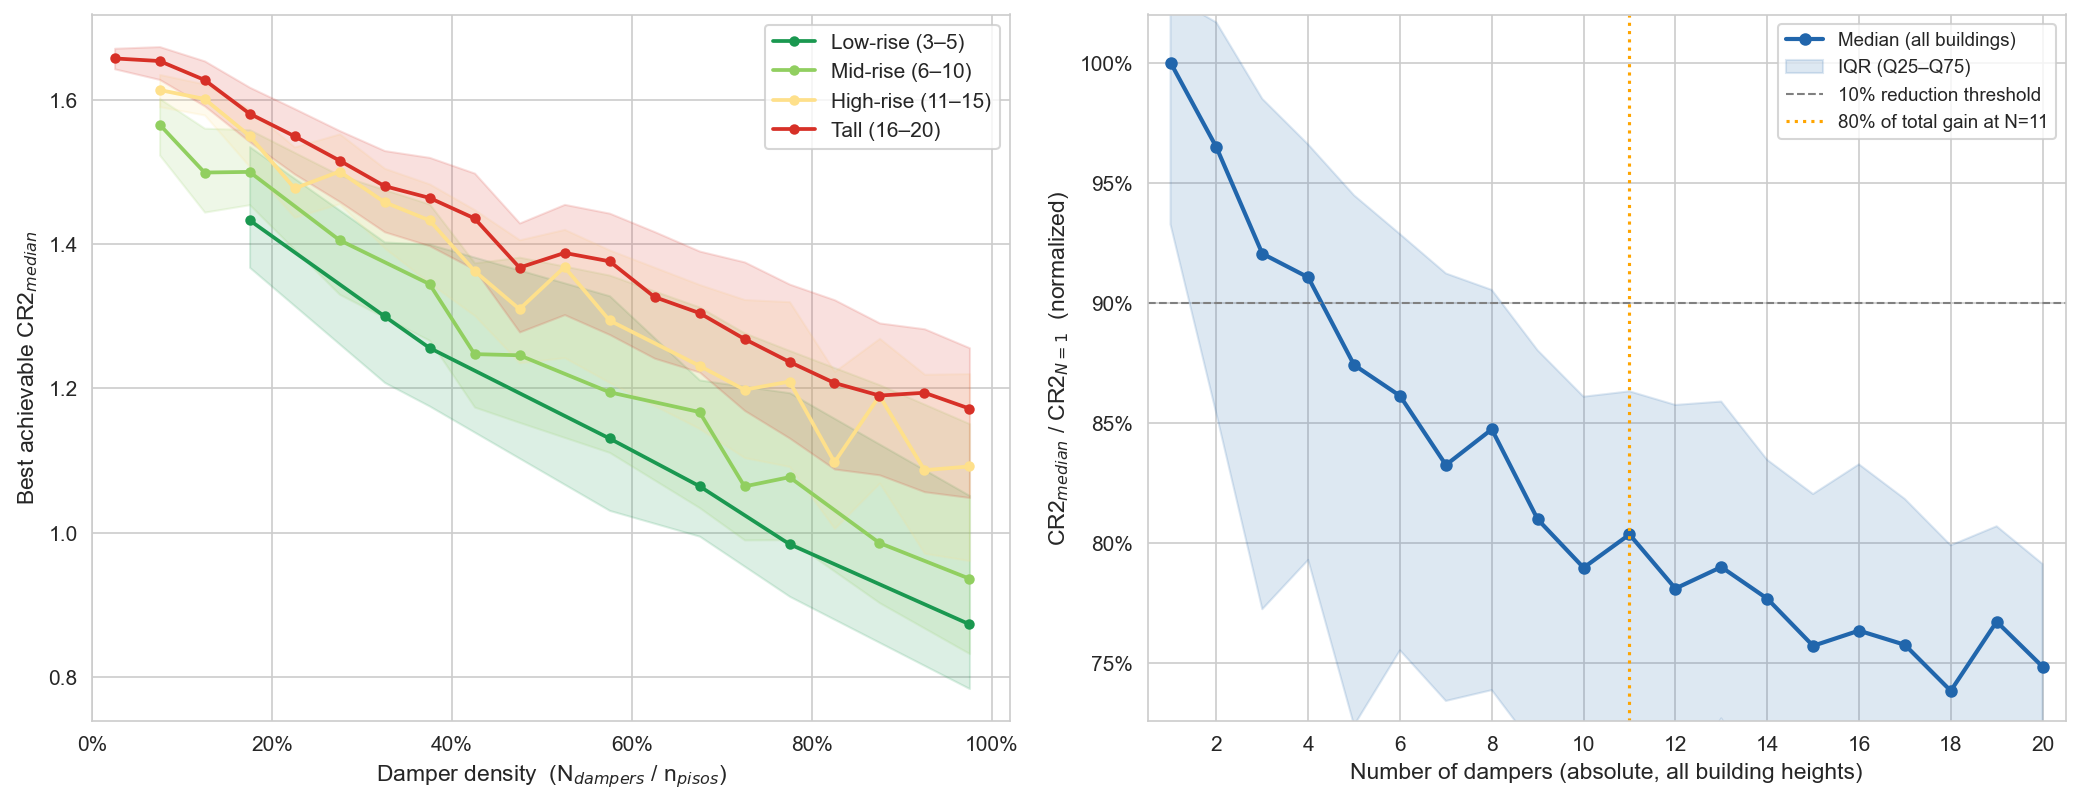
\includegraphics[width=\linewidth]{figs/F5_diminishing_returns.png}
\caption{Izquierda: mejor $\CR{med}$ alcanzable vs.\ densidad de cobertura
$\etad$, estratificado por altura del edificio (mediana $\pm$ IQR). Derecha:
$CR_2$ normalizado vs.\ $\nd$ absoluto para todos los edificios (nota: confundido
con la altura; el panel izquierdo provee la comparación apropiada).}
\label{fig:decreciente}
\end{figure}

\begin{figure}[htbp]
\centering
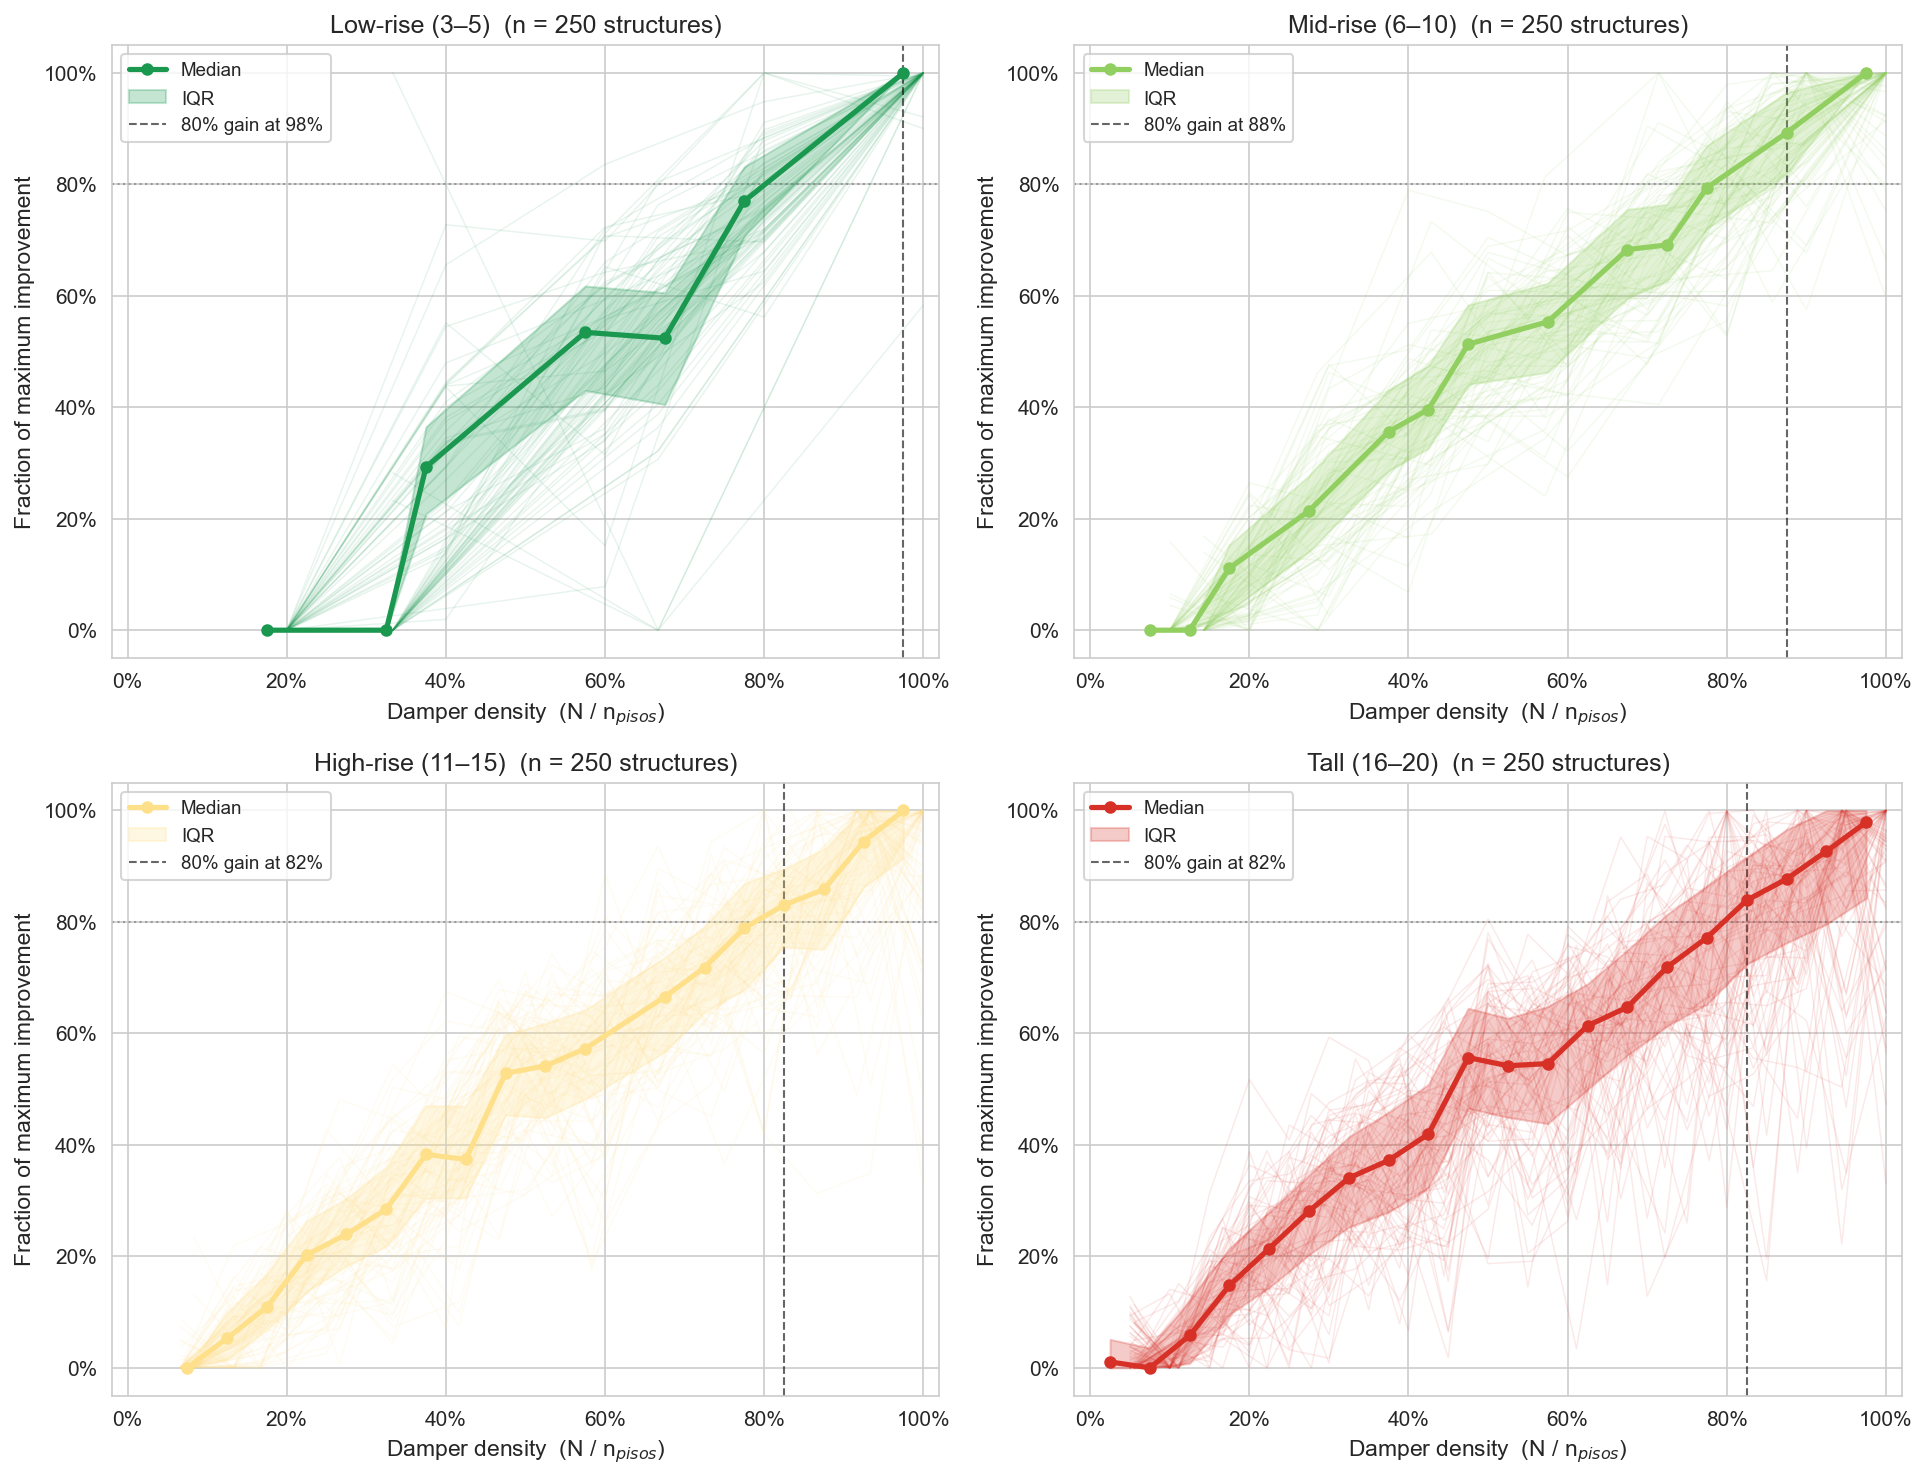
\includegraphics[width=\linewidth]{figs/F6_within_structure_curves.png}
\caption{Curvas de rendimiento decreciente intra-estructura por grupo de altura.
Cada línea delgada representa una estructura individual; la línea gruesa es la
mediana del grupo $\pm$ IQR. Línea punteada vertical: densidad a la que se
alcanza el 80\,\% de la ganancia máxima.}
\label{fig:curvas_internas}
\end{figure}

\subsection{Interacción entre Cantidad de Amortiguadores y Momento Friccional}
\label{sec:results:interaccion}

La \cref{fig:mapa_calor} presenta un mapa de calor bidimensional del $CR_2$
mediano en función de $\nd$ y $\Mf$ binados, estratificado por tres grupos de
altura (\cref{fig:mapa_calor}). El análisis estratificado revela patrones
diferenciados que el mapa global no captura.

En los tres grupos, baja densidad combinada con $\Mf \leq 100$\KM produce los
valores más altos de $CR_2$ (peor desempeño), confirmando que ambas variables
actúan como restricciones mínimas necesarias. Sin embargo, el peso relativo de
cada variable varía con la altura del edificio. En marcos bajos (3--5 pisos)
tanto $\nd$ como $\Mf$ contribuyen de forma comparable: incrementar $\nd$ de
1--2 a 3--4 con $\Mf \in [200,\,300]$\KM reduce $CR_2$ de 1{,}46 a 1{,}12,
y aumentar $\Mf$ de 100 a 300\KM con $\nd$ fijo produce reducciones similares,
lo que indica una relación de sustitución efectiva entre cantidad y capacidad.
En marcos de altura media y alta (6--20 pisos) $\nd$ domina de forma
progresivamente más clara: a cualquier nivel de $\nd$, incrementar $\Mf$ sigue
aportando mejoras ($\Delta CR_2 \approx 0{,}37$--$0{,}46$ en el rango completo
de $\Mf$), pero el efecto de añadir dispositivos supera sistemáticamente al de
aumentar la capacidad por dispositivo. En ningún grupo se observa insensibilidad
a $\Mf$ a alta cobertura: incluso con $\nd \geq 11$, la diferencia entre
$\Mf < 100$\KM y $\Mf > 400$\KM es de 0{,}46 unidades de $CR_2$ para marcos
medios y 0{,}37 para marcos altos.

Las configuraciones óptimas identificadas por el modelo ML para las 1\,000
estructuras se concentran en $\Mf \in [300,\,460]$\KM (mediana 400\KM,
IQR~[269,\,456]\KM) con fracciones de cobertura predominantemente iguales o
cercanas a la unidad ($\tilde{\eta}_{0{,}50} = 1{,}0$).

\begin{figure}[htbp]
\centering
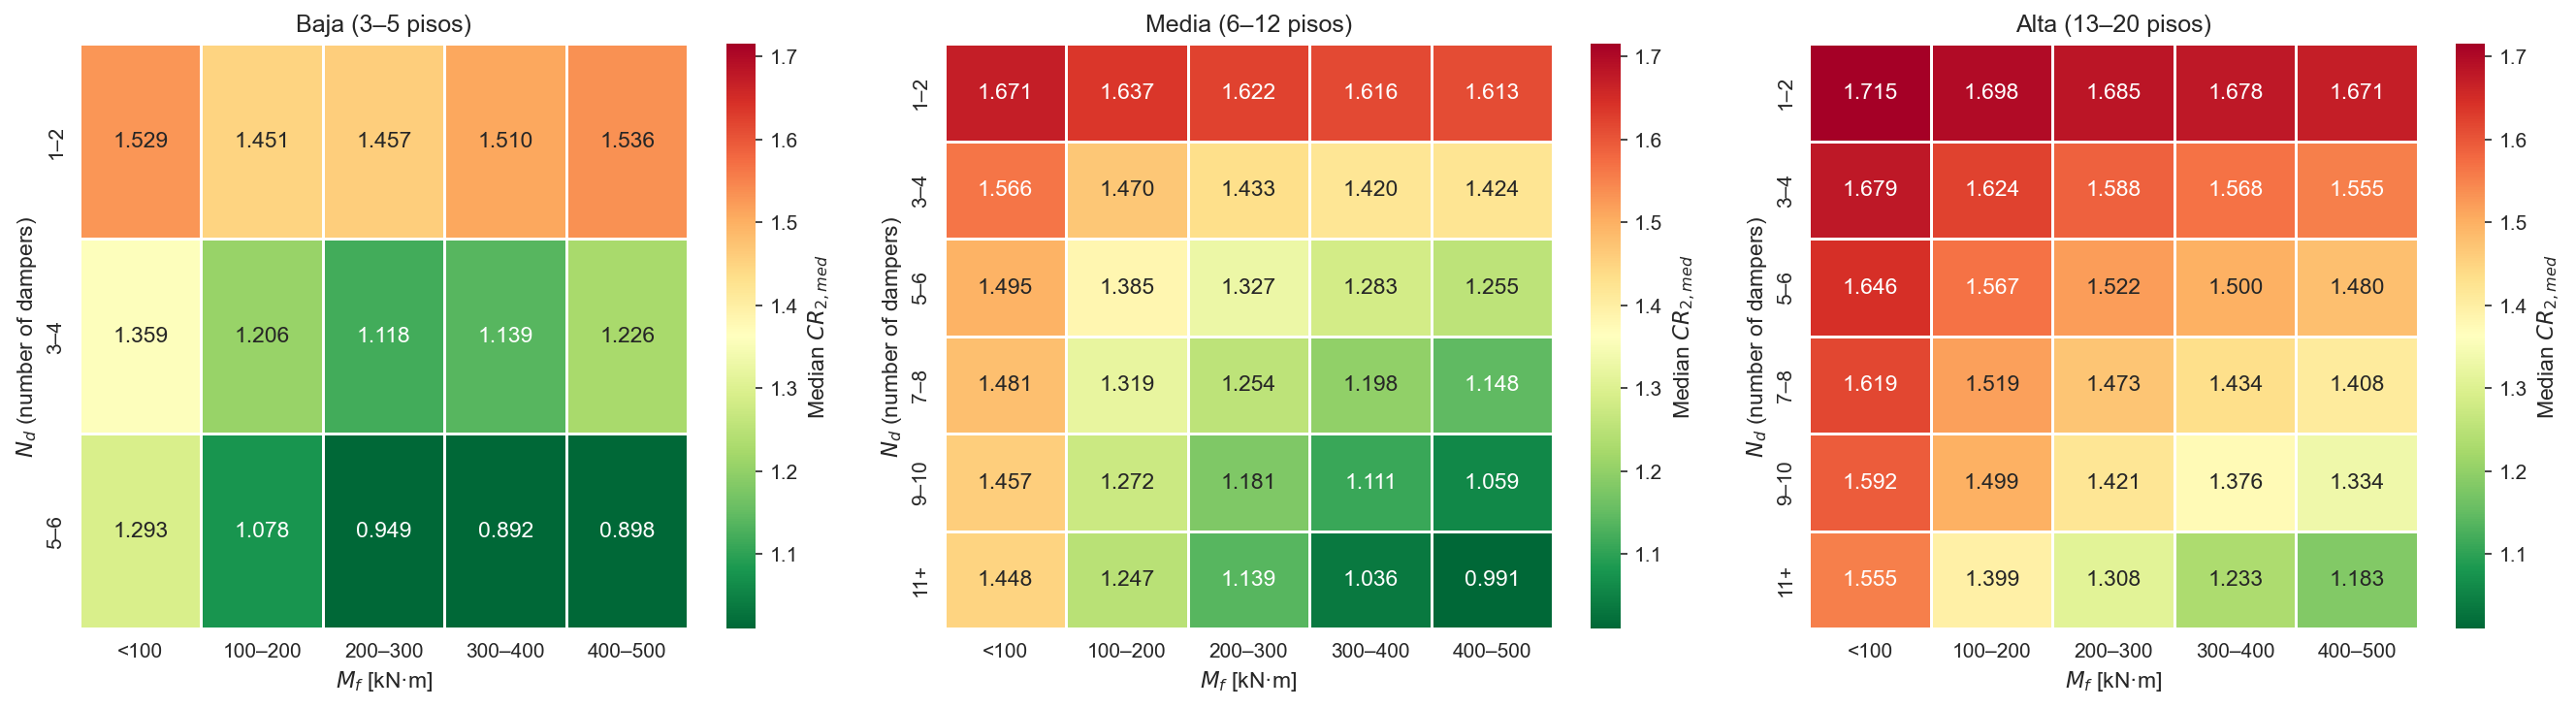
\includegraphics[width=\linewidth]{figs/F7_interaction_heatmap.png}
\caption{Izquierda: $CR_2$ mediano en función de bins de $\nd$ y bins de $\Mf$
(kN$\cdot$m), promediado sobre todas las estructuras y registros. Derecha:
$\nd$ óptimo vs.\ $\Mf$ para la mejor configuración de cada estructura (color:
$\CR{med}$ alcanzado).}
\label{fig:mapa_calor}
\end{figure}

\subsection{Convergencia del Diseño entre Escenarios Sísmicos}
\label{sec:results:convergencia}

La \cref{fig:convergencia} examina si un único diseño óptimo de AFR resulta
robusto entre los tres escenarios sísmicos. Para cada una de las 1\,000
estructuras se comparó el $\nd$ óptimo predicho bajo cada variable objetivo. La
distribución de $\nd$ recomendado es consistente entre escenarios: los escenarios
de mediana y P10 producen recomendaciones casi idénticas en la mayoría de las
estructuras. El escenario P90 tiende a recomendar un $\nd$ ligeramente mayor para
los edificios más altos, pero la discrepancia absoluta $|\nd^{\mathrm{P90}} -
\nd^{\mathrm{med}}|$ se mantiene por debajo de 2 para más del 80\,\% de las
estructuras. Esto implica que un diseño optimizado para el escenario de mediana
proporciona protección casi óptima frente a toda la variabilidad sísmica capturada
por el ensemble de ocho registros.

\begin{figure}[htbp]
\centering
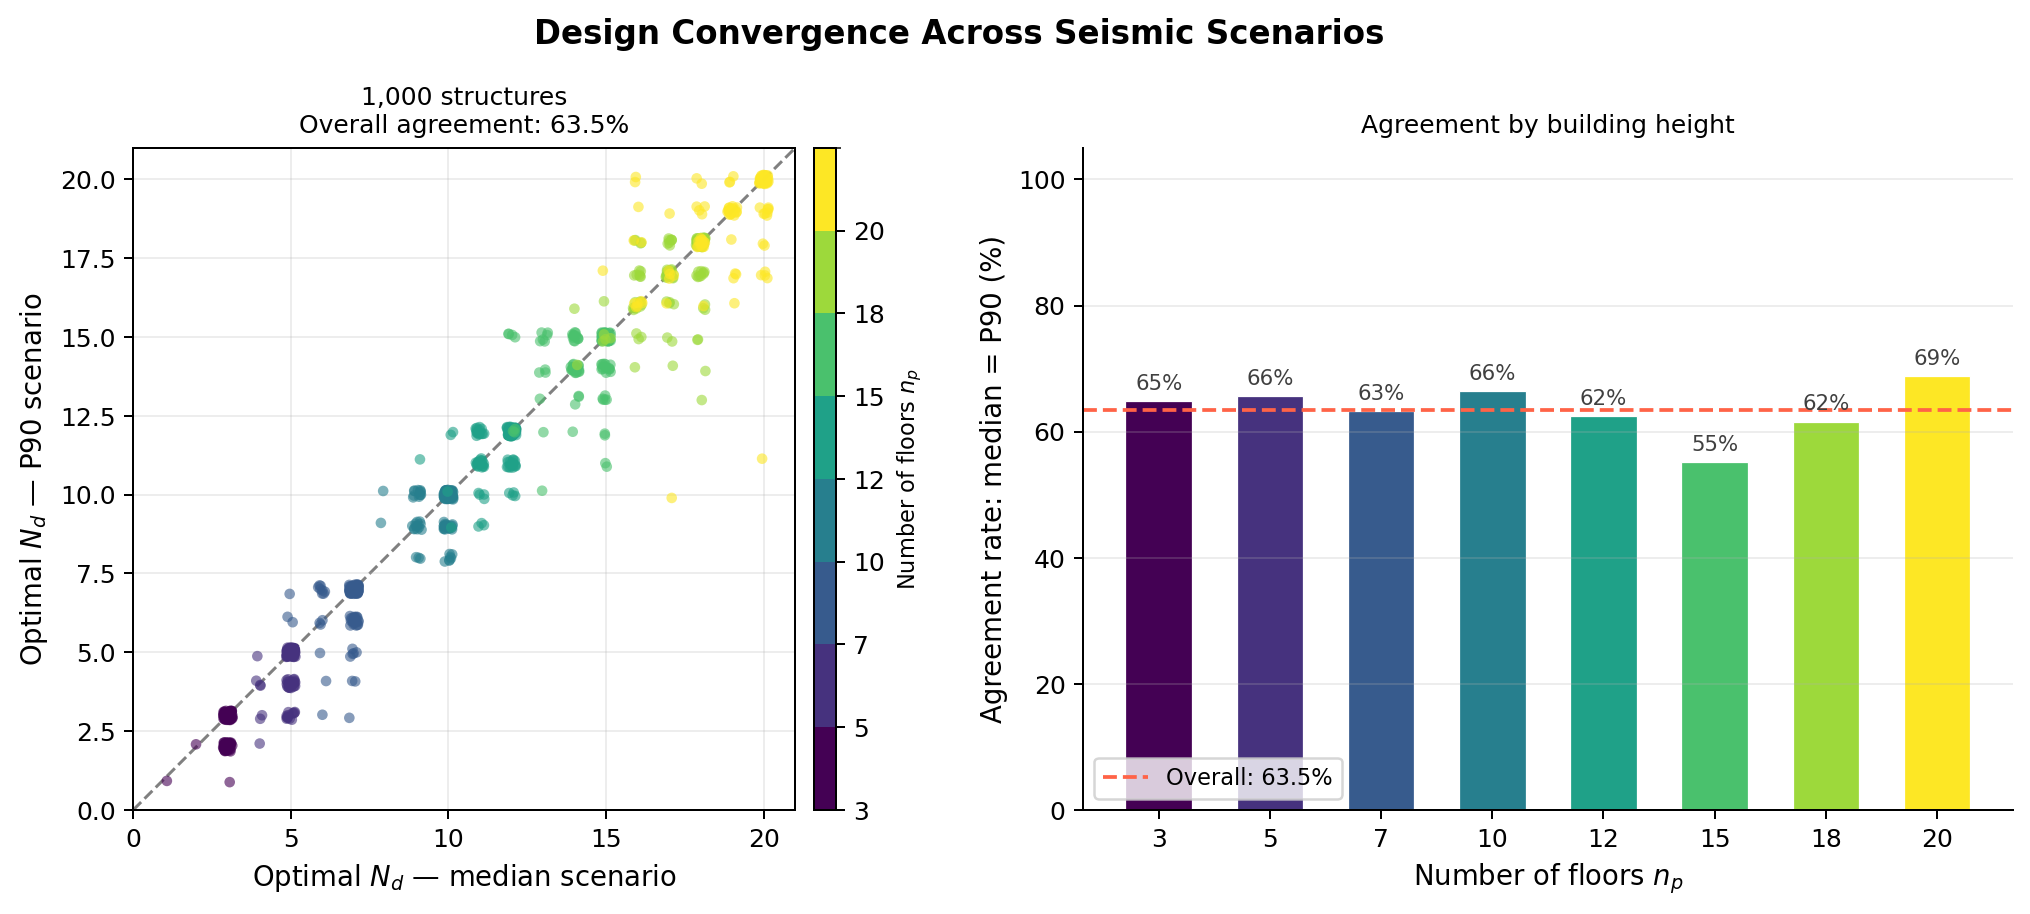
\includegraphics[width=\linewidth]{figs/F8_convergence_extended.png}
\caption{Izquierda: distribución del $\nd$ recomendado por escenario sísmico en
las 1\,000 estructuras. Derecha: tasa de acuerdo y discrepancia absoluta media
$|\nd^{\mathrm{P90}} - \nd^{\mathrm{med}}|$ por altura de edificio $\np$.}
\label{fig:convergencia}
\end{figure}

%%═══════════════════════════════════════════════════════════════════════════
\section{Discusión}
\label{sec:discussion}
%%═══════════════════════════════════════════════════════════════════════════

\subsection{La Densidad como Parámetro Gobernante de Diseño}

La densidad de cobertura $\etad$ emerge como el predictor dominante de $CR_2$
($r = -0{,}73$) y su dominancia es robusta: el análisis de dominancia
estocástica confirma que esta jerarquía se mantiene en los ocho registros
sísmicos con independencia de las demás variables de diseño
(Sección~\ref{sec:results:decreciente}). Con base en el análisis del umbral
del 80\,\% de ganancia máxima, se deriva la siguiente recomendación de diseño:
$\etad \geq 0{,}85$ para marcos de mediana y gran altura (6--20 pisos), y
$\etad \geq 0{,}90$ para marcos de baja altura (3--5 pisos), donde el impacto
proporcional de cada dispositivo adicional es mayor.

\subsection{Interacción entre Momento Friccional y Cobertura}

El análisis del mapa de calor (\cref{fig:mapa_calor}) revela una relación de
sustitución entre $\nd$ y $\Mf$ a niveles de cobertura intermedios: duplicar
$\Mf$ con un conteo fijo produce reducciones de $CR_2$ similares a incrementar
$\nd$ en dos pisos. Esta interacción no queda capturada por el análisis de
correlación marginal y motiva el uso de modelos ML de ensemble que representan
explícitamente las interacciones no lineales entre características. A alta
cobertura ($\etad \geq 0{,}75$), el desempeño se vuelve relativamente insensible
al valor específico de $\Mf$ dentro del rango [200,\,500]\KM, y el rango óptimo
identificado por ML, $\Mf \in [300,\,460]$\KM, es consistente con el óptimo
$\Mf = 257{,}9$\,kips$\cdot$in $\approx 290$\KM reportado por
\citet{Jarrahi2020jbe} para un MARM de un piso bajo una excitación de mayor
intensidad.

\subsection{Robustez entre Escenarios}

El alto nivel de acuerdo entre las recomendaciones de diseño de los escenarios
de mediana y P90 (\cref{fig:convergencia}) implica que no es necesario resolver
problemas de optimización separados para diferentes niveles de peligro sísmico
cuando el objetivo es identificar el $\nd$ óptimo. El enfoque multi-registro
aborda directamente la limitación de los estudios de optimización con un único
registro \citep{Jarrahi2020jbe,Jarrahi2020sdee}, capturando la variabilidad
registro-a-registro en las estadísticas P10, mediana y P90, lo que hace a las
recomendaciones ML inherentemente robustas frente a la incertidumbre en la
selección de acelerogramas.

\subsection{Limitaciones}

Se deben reconocer las siguientes limitaciones. (i)~Los modelos estructurales son
marcos cortantes elásticos idealizados; la interacción no lineal marco--AFR no
queda capturada explícitamente. (ii)~Los ocho acelerogramas, aunque sísmicamente
diversos, pueden no representar todos los entornos tectónicos relevantes.
(iii)~La validación del modelo se basa únicamente en validación cruzada; un
conjunto de prueba independiente proporcionaría una evaluación de generalización
más rigurosa. (iv)~Se asume un valor uniforme de $\Mf$ por estructura; las
distribuciones de $\Mf$ específicas por piso pueden ser preferibles en la
práctica. (v)~No se incorpora ninguna función de costo, por lo que la
optimización económica de la fracción de cobertura no se aborda.

%%═══════════════════════════════════════════════════════════════════════════
\section{Conclusiones}
\label{sec:conclusions}
%%═══════════════════════════════════════════════════════════════════════════

Las siguientes conclusiones principales se derivan del análisis de
$\approx$434\,000 simulaciones tiempo-historia no lineales sobre 1\,000
configuraciones estructurales diversas y ocho registros sísmicos reales:

\begin{enumerate}

\item \textbf{Precisión del modelo sustituto ML.}
XGBoost y Random Forest alcanzaron $\Rsq$ de 0{,}92--0{,}93 para $\CR{med}$ y
$\CR{P10}$, y 0{,}84 para $\CR{P90}$. Los modelos de ensemble redujeron el error
de predicción en $\approx$49\,\% respecto a los baselines lineales, cuantificando
la estructura no lineal de la relación diseño--desempeño.

\item \textbf{La densidad de amortiguadores es la variable de diseño primaria.}
La fracción de cobertura $\etad = \nd/\np$ es el predictor más influyente
($r = -0{,}73$), superando ampliamente al número absoluto de amortiguadores
($r = -0{,}45$). Las guías de diseño para AFR deben expresarse en términos de
$\etad$, no de $\nd$.

\item \textbf{Umbral de rendimiento decreciente: $\etad \approx 0{,}85$.}
El análisis intra-estructura revela que el 80\,\% de la reducción máxima de
$CR_2$ se alcanza con $\etad \approx 0{,}85$ para marcos de mediana y gran
altura (6--20~pisos) y con $\etad \approx 0{,}95$ para marcos de baja altura
(3--5~pisos). Estos umbrales proveen criterios prácticos de costo-efectividad
para el despliegue de AFR.

\item \textbf{Rango óptimo del momento friccional.}
En las 1\,000 estructuras analizadas, el $\Mf$ óptimo identificado por ML se
concentra en [300,\,460]\KM (mediana 400\KM). Para $\etad \geq 0{,}75$,
$CR_2$ es relativamente insensible al valor específico de $\Mf$ dentro de
[200,\,500]\KM, por lo que la fracción de cobertura es el parámetro de diseño
más crítico.

\item \textbf{Robustez entre escenarios.}
El $\nd$ óptimo recomendado por los escenarios de mediana y P90 difiere en menos
de 2~pisos en el 80\,\% de las estructuras analizadas, confirmando que un diseño
optimizado para la mediana proporciona protección casi óptima frente a toda la
variabilidad sísmica del ensemble de ocho registros.

\item \textbf{Trabajo futuro.}
Las extensiones deben incorporar comportamiento inelástico del marco,
distribuciones de $\Mf$ específicas por piso, restricciones de costo de
instalación y suites de registros sísmicos más amplias que representen diferentes
entornos tectónicos. La validación experimental para configuraciones multi-piso
y la integración de los modelos entrenados en una herramienta de diseño
interactiva constituyen direcciones inmediatas de investigación.

\end{enumerate}

%%═══════════════════════════════════════════════════════════════════════════
\bibliographystyle{elsarticle-harv}
\bibliography{references}

\end{document}
